\documentclass{article}
\usepackage{../arxiv}
\usepackage[no-math]{fontspec}
\usepackage{mathptmx}
\setmainfont{Sarabun}[Path=fonts/, Extension=.ttf, UprightFont=*-Regular, BoldFont=*-Bold,
  ItalicFont=*-Italic, BoldItalicFont=*-BoldItalic, Script=Thai]
\XeTeXlinebreaklocale "th"
\XeTeXlinebreakskip = 0pt plus 1pt
\linespread{1.12}
\usepackage{microtype}
\emergencystretch=3em
\usepackage{amsmath, amssymb, amsthm, mathtools, bm}
\usepackage{graphicx, booktabs, array, float, placeins}
\graphicspath{{../figures/}}
\usepackage{xcolor}
\usepackage[font=small, labelfont=bf, labelsep=period]{caption}
\usepackage{enumitem}
\setlist{itemsep=2pt, topsep=3pt}
\usepackage{tikz}
\usetikzlibrary{positioning, calc, arrows.meta}
\usepackage{listings}
\usepackage[round, authoryear]{natbib}
\usepackage[unicode, colorlinks=true, linkcolor=blue!45!black, citecolor=blue!45!black, urlcolor=blue!45!black]{hyperref}
\usepackage{xurl}
\hypersetup{pdftitle={ล็อกดาวน์ในฐานะวันหยุดบางส่วน}, pdfauthor={ธนัชชนม์ จงมั่นคง},
  pdfkeywords={Prophet, holiday effects, COVID-19, temporal aggregation, Thailand}}
\renewcommand{\shorttitle}{ล็อกดาวน์ในฐานะวันหยุดบางส่วน}
\renewcommand{\headeright}{ฉบับก่อนตีพิมพ์}
\renewcommand{\undertitle}{ฉบับก่อนตีพิมพ์ (Preprint)}

\renewcommand{\figurename}{รูปที่}
\renewcommand{\tablename}{ตารางที่}
\renewcommand{\refname}{เอกสารอ้างอิง}
% arxiv.sty abstract with a settable heading: \begin{abstract}[บทคัดย่อ]
\renewenvironment{abstract}[1][Abstract]{\centerline{\large\bfseries\scshape #1}\begin{quote}}{\end{quote}}
\newcommand{\thaikeywords}[1]{{\def\keywordname{{\bfseries คำสำคัญ}}\keywords{#1}}}
\theoremstyle{definition}
\newtheorem{proposition}{ข้อเสนอ}
\newtheorem{corollary}{บทแทรก}
\newcommand{\HESI}{\mathrm{HESI}}
\lstset{language=Python, basicstyle=\ttfamily\scriptsize, keywordstyle=\color{blue!60!black}\bfseries,
  commentstyle=\color{green!40!black}\itshape, stringstyle=\color{red!50!black}, frame=single,
  rulecolor=\color{black!25}, breaklines=true, columns=fullflexible, showstringspaces=false,
  backgroundcolor=\color{black!2}, xleftmargin=2pt, xrightmargin=2pt}

\title{ล็อกดาวน์ในฐานะ “วันหยุดบางส่วน”:\\ การถ่ายโอนผลกระทบการหยุดงานจากสงกรานต์และตรุษจีน\\ เพื่อพยากรณ์มูลค่าการส่งออกรายเดือนของไทยผ่านช่วงโควิด-19 ด้วย Prophet}
\author{\textbf{ธนัชชนม์ จงมั่นคง}\thanks{ผลเชิงปริมาณทั้งหมดในฉบับนี้มาจาก\textbf{การศึกษาแบบจำลอง (simulation study)} อนุกรมมูลค่าส่งออกเป็นข้อมูลจำลองที่ปรับสเกลให้ใกล้เคียงการส่งออกของไทย ส่วนปฏิทินวันหยุด ดัชนี OxCGRT และ Google Mobility เป็นข้อมูลจริง การยืนยันกับข้อมูลส่งออกจริงทำได้ด้วยคำสั่ง \texttt{real} ในโค้ดที่แนบ (ภาคผนวก ก) รายการเอกสารอ้างอิงรวบรวมโดยไม่ได้ตรวจกับฐานข้อมูลบรรณานุกรม จึงต้องตรวจสอบก่อนเผยแพร่}}
\date{7 พฤศจิกายน 2569}

\begin{document}
\maketitle

\begin{abstract}[บทคัดย่อ]
\noindent ช็อกจากโควิด-19 ทำให้อนุกรมมูลค่าการส่งออกรายเดือนของไทยมีช่วงที่หดตัวและฟื้นตัวผิดปกติ แบบจำลองพยากรณ์จึงเรียนรู้แนวโน้มและฤดูกาลที่บิดเบี้ยว และไม่มีพารามิเตอร์ใดที่ใช้คาดการณ์ผลของล็อกดาวน์ได้ก่อนที่จะเกิดขึ้น งานวิจัยนี้เสนอกรอบ \emph{Holiday-Equivalent Stoppage} (HES) ซึ่งมองล็อกดาวน์เป็น “วันหยุดบางส่วน” โดยให้ Prophet เรียนรู้ผลของการหยุดงานจากวันหยุดที่เกิดซ้ำทุกปี ได้แก่วันหยุดราชการไทยรวมสงกรานต์ (ช่องทางในประเทศ) และหน้าต่างตรุษจีน (ช่องทางคู่ค้า) ผ่านตัวแปรร่วมเพียงตัวเดียวต่อช่องทาง แล้วถ่ายโอนผลนั้นไปยังช่วงโควิดด้วยดัชนี HESI ซึ่งบอกว่าวันหนึ่งเทียบเท่าวันหยุดกี่ส่วน ดัชนีนี้คำนวณจากการลดลงของการเดินทางไปที่ทำงาน (Google Mobility) หารด้วยการลดลงในวันหยุดจริง บทความวิเคราะห์เงื่อนไขที่ทำให้การถ่ายโอนได้ผล อคติจากการรวมข้อมูลรายวันเป็นรายเดือนตามอสมการของ Jensen ปัญหาการระบุค่าเมื่อมีเพียงข้อมูลรายเดือน และเหตุที่แบบจำลองต้นไม้ถ่ายโอน “ปริมาณ” ไม่ได้ จากนั้นประเมินด้วยการจำลอง Monte Carlo จำนวน 30 รอบที่ใช้ปฏิทินวันหยุดและตัวขับเคลื่อนโควิดจริง ผลพบว่า (1)~เมื่อปริมาณถูกต้อง Prophet รายวันลด MAPE ช่วงปี 2020--2021 จาก 26.0\% เหลือ 7.8\% (2)~การเปิดผลวันหยุดตลอดทั้งเดือนแบบ binary ช่วยได้น้อย (22.7\%) และการใช้ดัชนี stringency ดิบทำให้แย่ลง (3)~ข้อมูลรายวันประมาณผลวันหยุดได้แม่นยำ ($\hat\beta_D=-0.80$ เทียบค่าจริง $-0.80$) ขณะที่ข้อมูลรายเดือนให้ค่าที่ถูกลดทอนและแกว่ง ($-0.54\pm0.13$) (4)~LightGBM ถ่ายโอนปริมาณไม่ได้เพราะเรียนรู้ความสัมพันธ์แบบสวิตช์ และ (5)~เมื่อปริมาณจาก mobility สูงเกินจริงสองเท่า การปรับเทียบจากสองเดือนแรกของล็อกดาวน์ลด MAPE จาก 13.0\% เหลือ 8.8\% ในช่วงปกติและช่วงหลังช็อก วิธีที่เรียบง่ายกว่า เช่น SARIMAX และการตัดช่วงช็อกออก ยังแข่งขันได้ดีหรือดีกว่า HES จึงเป็นเครื่องมือสำหรับช่วงช็อกที่วัดปริมาณได้ ไม่ใช่สูตรสำเร็จสำหรับทุกช่วงเวลา
\end{abstract}

\thaikeywords{Prophet \and ผลของวันหยุด \and โควิด-19 \and intervention analysis \and การถ่ายโอน \and การรวมข้อมูลตามเวลา \and การส่งออกของไทย \and LightGBM}

\noindent{\bfseries รหัส JEL}\enspace C15, C22, C53, F17

\begin{abstract}
\noindent \textbf{Lockdowns as Partial Holidays: Transferring Work-Stoppage Effects Learned from Songkran and Chinese New Year to Forecast Thailand's Monthly Exports through COVID-19.}
The COVID-19 shock created an abnormal collapse-and-rebound episode in Thailand's monthly export series. Forecasting models learn distorted trends and seasonality from it, and none of their parameters can anticipate a lockdown before it is observed. We propose the \emph{Holiday-Equivalent Stoppage} (HES) framework, which treats a lockdown as a \emph{partial holiday}. Prophet learns the work-stoppage effect from holidays that recur every year (Thai public holidays including Songkran for the domestic channel, the Chinese New Year window for the partner channel) through one shared regressor per channel, and transfers it to the pandemic through a Holiday-Equivalent Stoppage Index (HESI): the drop in workplace mobility relative to the drop on actual holidays. We derive when the transfer works, the Jensen bias from aggregating daily effects to months, the identification problem with monthly-only data, and why tree ensembles cannot transfer a dose. A Monte Carlo study with 30 replications, built on the real Thai holiday calendar and real OxCGRT and Google Mobility drivers, shows that (i) with the right dose, daily Prophet cuts the 2020--2021 MAPE from 26.0\% to 7.8\%; (ii) switching the holiday effect on for whole months helps little (22.7\%) and raw stringency makes forecasts worse; (iii) daily data recover the holiday effect precisely ($\hat\beta_D=-0.80$ vs.\ $-0.80$) whereas monthly data give attenuated, noisy estimates ($-0.54\pm0.13$); (iv) LightGBM learns an on/off switch rather than a dose-response; and (v) when the mobility dose overstates the true stoppage two-fold, calibrating it on the first two lockdown months lowers MAPE from 13.0\% to 8.8\%. In normal and post-shock periods simpler approaches (SARIMAX, masking the shock window) remain competitive or better, so HES is a tool for measurable shocks rather than a universal accuracy gain.
\end{abstract}

\keywords{Prophet \and holiday effects \and COVID-19 \and intervention analysis \and transfer \and temporal aggregation \and Thai exports \and LightGBM}

\section{บทนำ}
การส่งออกสินค้าเป็นเครื่องยนต์สำคัญของเศรษฐกิจไทย ตัวเลขมูลค่าการส่งออกรายเดือนจึงถูกติดตามและพยากรณ์อย่างต่อเนื่องโดยหน่วยงานภาครัฐ ธนาคารกลาง และภาคเอกชน ในช่วงปี 2020--2022 การระบาดของโควิด-19 ทำให้อนุกรมนี้มีพฤติกรรมที่ไม่เคยปรากฏมาก่อน ทั้งการหดตัวรุนแรงในไตรมาสที่สองของปี 2020 และการฟื้นตัวแข็งแรงในปี 2021 สำหรับผู้พยากรณ์ ช่วงเวลานี้สร้างปัญหาสามชั้น ชั้นแรก แบบจำลองที่เรียนแนวโน้มและฤดูกาลจากข้อมูลจะถูกดึงให้บิดเบี้ยวตามช่วงช็อก ชั้นที่สอง ตัวแปรล้าหลัง (lag features) ที่แบบจำลองเชิงเครื่องจักรใช้จะพาความผิดปกติไปปนเปื้อนการพยากรณ์ในปีถัดไป ชั้นที่สามซึ่งเป็นปัญหาพื้นฐานที่สุด คือแบบจำลองไม่มีกลไกใดที่คาดการณ์ผลของล็อกดาวน์ครั้งใหม่ได้ก่อนจะเห็นข้อมูลของมัน

วิธีมาตรฐานที่ใช้รับมือกับช็อก ได้แก่ intervention analysis ด้วยตัวแปรหุ่น \citep{box1975intervention} การประมาณผลของค่าผิดปกติร่วมกับพารามิเตอร์แบบจำลอง \citep{chen1993joint} การตัดช่วงช็อกออกจากข้อมูลฝึก และการใส่ช่วงล็อกดาวน์เป็น “วันหยุดครั้งเดียว” ใน Prophet ตามที่เอกสารของ Prophet แนะนำ \citep{prophetshocks} ทุกวิธีมีจุดร่วมกัน คือต้องเห็นช็อกก่อนจึงจะประมาณผลได้ ส่วนแบบจำลองต้นไม้ เช่น LightGBM \citep{ke2017lightgbm} ซึ่งทำผลงานโดดเด่นในการแข่งขัน M5 \citep{makridakis2022m5} มีข้อจำกัดเพิ่มอีกชั้น คือไม่สามารถ extrapolate ไปยังค่าของตัวแปรที่อยู่นอกช่วงข้อมูลฝึก \citep{januschowski2022trees}

งานวิจัยนี้ตั้งต้นจากข้อสังเกตว่า ในแง่ของการผลิตและการขนส่งสินค้า ล็อกดาวน์มีลักษณะคล้าย\emph{วันหยุด} ประเทศไทยมี “การทดลองตามธรรมชาติ” ของการหยุดงานทั่วประเทศทุกปี คือเทศกาลสงกรานต์และวันหยุดราชการอื่น ๆ และมีการหยุดงานของคู่ค้าหลักทุกปี คือเทศกาลตรุษจีน วันหยุดเหล่านี้เกิดซ้ำกว่าสิบปีก่อนโควิด ข้อมูลจึงเพียงพอให้แบบจำลองเรียนรู้ว่า “การหยุดงานหนึ่งวันทำให้มูลค่าส่งออกหายไปเท่าใด” หากวัดได้ว่าวันหนึ่งในช่วงล็อกดาวน์เทียบเท่าวันหยุดกี่ส่วน แบบจำลองก็พยากรณ์ผลของล็อกดาวน์ได้โดยไม่ต้องมีพารามิเตอร์ใหม่

อย่างไรก็ดี การนำแนวคิดนี้ไปใช้แบบตรงไปตรงมา คือ “เปิดผลวันหยุดตลอดทั้งเดือนในช่วงโควิด” มีความเสี่ยง เพราะวันล็อกดาวน์ส่วนใหญ่ไม่ได้หยุดงานเท่าวันสงกรานต์ งานนี้จึงแทนสวิตช์เปิด/ปิดด้วย\emph{ปริมาณ} (dose) ที่วัดได้ และมีส่วนร่วมทางวิชาการดังนี้
\begin{enumerate}
\item เสนอกรอบ HES ที่ใช้ตัวแปรร่วมหนึ่งตัวต่อช่องทาง (ในประเทศและคู่ค้า) ใน Prophet และดัชนี HESI ที่สร้างจากข้อมูล mobility จริงโดยใช้วันหยุดเป็นหน่วยอ้างอิง
\item วิเคราะห์ว่าเมื่อใดการถ่ายโอนจึงได้ผล แสดงอคติจากการรวมข้อมูลรายวันเป็นรายเดือนตามอสมการของ Jensen ปัญหาการระบุค่าเมื่อสงกรานต์ตรงกับฤดูกาลเดือนเมษายน และกลไกที่ทำให้แบบจำลองต้นไม้ล้มเหลว พร้อมวิธีแก้อคติสำหรับผู้ที่มีเพียงข้อมูลรายเดือน (aggregation correction; AC)
\item ประเมินด้วยการจำลอง Monte Carlo ที่ใช้ปฏิทินวันหยุดไทยตามที่หยุดจริง ดัชนี OxCGRT และ Google Mobility จริง ภายใต้สถานการณ์ที่การถ่ายโอนสมบูรณ์และสถานการณ์ที่สมจริงกว่า ครอบคลุมช่วงปกติ ช่วงช็อก และหลังช็อก
\item เปิดเผยโค้ดและขั้นตอนสำหรับนำไปใช้กับข้อมูลส่งออกจริง
\end{enumerate}
หัวข้อที่ 2 ทบทวนงานที่เกี่ยวข้อง หัวข้อที่ 3 เสนอกรอบแนวคิดและผลเชิงทฤษฎี หัวข้อที่ 4 อธิบายข้อมูลและการออกแบบการทดลอง หัวข้อที่ 5 รายงานผล หัวข้อที่ 6 อภิปรายข้อจำกัดและแนวทางนำไปใช้ และหัวข้อที่ 7 สรุป

\section{งานวิจัยที่เกี่ยวข้อง}
\paragraph{ผลของปฏิทินและวันหยุดที่เคลื่อนที่}
\citet{bell1983calendar} วางกรอบการสร้างแบบจำลองผลของจำนวนวันทำการและวันหยุดในอนุกรมรายเดือน ซึ่งต่อมาเป็นส่วนหนึ่งของโปรแกรมปรับฤดูกาล X-12-ARIMA \citep{findley1998x12} ที่ใช้ตัวแปรถดถอยสำหรับวันหยุดที่เปลี่ยนวันทุกปี เช่น อีสเตอร์ สำหรับเอเชีย ตรุษจีนซึ่งตกเดือนมกราคมหรือกุมภาพันธ์สลับกันทำให้ตัวเลขรายเดือนแกว่งอย่างมีนัยสำคัญ \citep{lin2003lunar} งานกลุ่มนี้แสดงว่าผลวันหยุดประมาณได้จากข้อมูลรายเดือนเมื่อวันหยุดเคลื่อนที่ แต่ไม่ได้นำผลนั้นไปอธิบายช็อกประเภทอื่น

\paragraph{ช็อกและค่าผิดปกติ}
Intervention analysis \citep{box1975intervention} และการประมาณผลค่าผิดปกติร่วมกับพารามิเตอร์ \citep{chen1993joint} ต้องสังเกตเหตุการณ์ก่อนจึงจะประมาณขนาดผลได้ ในบริบทโควิด \citet{lenza2022var} ปรับความแปรปรวนของ VAR หลังเดือนมีนาคม 2020 เพื่อไม่ให้ช่วงช็อกครอบงำการประมาณค่า ส่วน \citet{foroni2022covid} ใช้บทเรียนจากวิกฤตการเงินโลกช่วยพยากรณ์การถดถอยและการฟื้นตัว วิธีเหล่านี้อาศัยเหตุการณ์ที่ “คล้ายกันในเชิงขนาด” ขณะที่งานนี้อาศัยเหตุการณ์ที่ “คล้ายกันในเชิงกลไก” และเกิดซ้ำทุกปี

\paragraph{Prophet}
\citet{taylor2018forecasting} เสนอแบบจำลองแยกองค์ประกอบ $y(t)=g(t)+s(t)+h(t)+\varepsilon_t$ ที่รองรับวันหยุดและตัวแปรถดถอยเพิ่มเติม จุดสำคัญคือ Prophet สร้างพารามิเตอร์แยกให้วันหยุดแต่ละชื่อ (และแต่ละวันในหน้าต่างของวันหยุดนั้น) ดังนั้นการตั้ง “covid” เป็นวันหยุดชื่อใหม่จะไม่เกิดการถ่ายโอนใด ๆ เพราะพารามิเตอร์ใหม่ไม่มีข้อมูลให้เรียนก่อนเกิดเหตุ

\paragraph{แบบจำลองต้นไม้}
Gradient boosting บนต้นไม้ตัดสินใจ \citep{ke2017lightgbm} ทำผลงานโดดเด่นในการแข่งขันพยากรณ์ขนาดใหญ่ \citep{makridakis2022m5} แต่ฟังก์ชันที่ได้เป็นแบบขั้นบันไดและคงที่นอกช่วงข้อมูลฝึก \citep{januschowski2022trees} งานนี้แสดงว่าข้อจำกัดดังกล่าวทำให้ต้นไม้ถ่ายโอน “ปริมาณ” ของการหยุดงานไม่ได้

\paragraph{ข้อมูลนโยบายและการเคลื่อนที่}
Oxford COVID-19 Government Response Tracker \citep{hale2021oxcgrt} ให้ดัชนีความเข้มงวดของมาตรการรายวัน และ Google COVID-19 Community Mobility Reports \citep{google2022mobility} ให้การเปลี่ยนแปลงของการเดินทางไปสถานที่ต่าง ๆ เทียบกับฐานก่อนโควิด \citet{sampi2020nowcasting} แสดงว่าข้อมูล mobility ช่วย nowcast กิจกรรมทางเศรษฐกิจได้ งานนี้ใช้ mobility ในบทบาทใหม่ คือเป็นตัวแปลงหน่วยจาก “ความเข้มของล็อกดาวน์” เป็น “จำนวนวันหยุดที่เทียบเท่า”

\paragraph{การรวมข้อมูลตามเวลา}
\citet{silvestrini2008aggregation} สำรวจผลของ temporal aggregation ต่อแบบจำลองอนุกรมเวลา งานนี้เพิ่มกรณีเฉพาะที่การแปลง log ทำให้ผลวันหยุดที่ “กระจุก” อยู่ไม่กี่วันกับผลล็อกดาวน์ที่ “กระจาย” ทั้งเดือนรวมเป็นรายเดือนต่างกัน

\section{กรอบแนวคิดและแบบจำลอง}
\subsection{แบบจำลองรายวันและตัวแปรการหยุดงานแบบใช้ร่วม}
ให้ $y_d$ คือมูลค่าส่งออกในวันที่ $d$ แบบจำลองบนสเกล log คือ
\begin{equation}\label{eq:daily}
\log y_d = g(t_d) + s(t_d) + w(d) + \beta_D\,x^D_d + \beta_P\,x^P_d + u_d ,
\end{equation}
เมื่อ $g$ คือแนวโน้มเชิงเส้นแบบมีจุดเปลี่ยน $s$ คือฤดูกาลรายปีแบบฟูเรียร์ $w$ คือผลของวันในสัปดาห์ และ $u_d$ คือความคลาดเคลื่อน ตัวแปรการหยุดงานของช่องทางในประเทศ ($D$) และช่องทางคู่ค้า ($P$) นิยามเป็น
\begin{align}
x^D_d &= H_d + (1-H_d)\,\min\{1,\ \lambda\,h_d\}, \label{eq:xd}\\
x^P_d &= C_d + (1-C_d)\,p_d , \label{eq:xp}
\end{align}
โดย $H_d=1$ ในวันหยุดราชการไทยที่หยุดจริง (รวมสงกรานต์และวันหยุดชดเชย) $C_d=1$ ในหน้าต่างตรุษจีน $[-1,+6]$ วันรอบวันแรกของเทศกาล $h_d\in[0,1]$ คือดัชนี HESI ของไทย $p_d\in[0,1]$ คือดัชนีการหยุดอุตสาหกรรมของจีนในหน่วยวันตรุษจีน และ $\lambda$ คือตัวคูณปริมาณ หัวใจของกรอบนี้คือ $\beta_D$ และ $\beta_P$ เป็นพารามิเตอร์\emph{ตัวเดียวกัน}ทั้งในวันหยุดและในวันล็อกดาวน์ ก่อนปี 2020 ตัวแปรทั้งสองมีค่าเป็น 0 หรือ 1 ตามวันหยุดเท่านั้น วันหยุดที่เกิดซ้ำทุกปีจึงระบุค่า $\beta$ ได้ก่อนเกิดโควิด และช่วงโควิดต้องการเพียงปริมาณ ไม่ต้องการพารามิเตอร์ใหม่ (รูปที่~\ref{fig:framework})

\begin{figure}[t]
\centering
\begin{tikzpicture}[node distance=3.5mm and 7mm, every node/.style={font=\footnotesize},
  box/.style={draw=#1!70!black, fill=#1!7, rounded corners=2pt, align=center, inner sep=3.5pt, text width=35mm},
  arr/.style={-{Stealth[length=2mm]}, thick, draw=black!55}]
\node[box=blue] (hol) {วันหยุดที่เกิดซ้ำทุกปี\\สงกรานต์ + วันหยุดราชการไทย\\$H_d=1$};
\node[box=orange, below=of hol] (cov) {ช่วงโควิดในไทย\\mobility ที่ลดลง ÷ ค่าอ้างอิงวันหยุด\\$h_d=\HESI_d\in[0,1]$};
\node[box=blue, below=7mm of cov] (cny) {ตรุษจีน\\หน้าต่าง $-1\ldots+6$ วัน\\$C_d=1$};
\node[box=orange, below=of cny] (cn) {จีนหยุดอุตสาหกรรม\\(episode ปี 2020 และ 2022)\\$p_d\in[0,1]$};
\node[box=green, text width=39mm] (xd) at ($(hol)!0.5!(cov)+(48mm,0)$) {ตัวแปรร่วมช่องทางในประเทศ\\$x^D_d=H_d+(1-H_d)\,\lambda h_d$};
\node[box=green, text width=39mm] (xp) at ($(cny)!0.5!(cn)+(48mm,0)$) {ตัวแปรร่วมช่องทางคู่ค้า\\$x^P_d=C_d+(1-C_d)\,p_d$};
\node[box=violet, text width=36mm] (pr) at ($(xd)!0.5!(xp)+(46mm,9mm)$) {Prophet รายวันบน $\log y_d$\\$g+s+w+\beta_D x^D_d+\beta_P x^P_d$};
\node[box=gray, text width=36mm, below=8mm of pr] (out) {รวมผลรายวัน\\$\Rightarrow$ พยากรณ์รายเดือน};
\draw[arr] (hol.east) -- node[above, sloped, font=\scriptsize] {เรียน $\beta$} (xd.west);
\draw[arr, dashed] (cov.east) -- node[below, sloped, font=\scriptsize] {ปริมาณ $\lambda$} (xd.west);
\draw[arr] (cny.east) -- node[above, sloped, font=\scriptsize] {เรียน $\beta$} (xp.west);
\draw[arr, dashed] (cn.east) -- node[below, sloped, font=\scriptsize] {ปริมาณ} (xp.west);
\draw[arr] (xd.east) -- (pr.west);
\draw[arr] (xp.east) -- (pr.west);
\draw[arr] (pr) -- (out);
\end{tikzpicture}
\caption{กรอบแนวคิด HES ผลของการหยุดงานเรียนจากวันหยุดที่เกิดซ้ำ (สีน้ำเงิน) ผ่านตัวแปรร่วม (สีเขียว) แล้วนำไปใช้กับช่วงโควิดด้วยปริมาณที่วัดได้ (สีส้ม) โดยไม่มีพารามิเตอร์ใหม่}
\label{fig:framework}
\end{figure}

\subsection{ดัชนี HESI: วันหนึ่งเทียบเท่าวันหยุดกี่ส่วน}
ให้ $m_d=\max\{0,-\text{workplaces}_d/100\}$ คือสัดส่วนที่การเดินทางไปที่ทำงานลดลงจากฐานก่อนโควิดตาม Google Mobility นิยาม
\begin{equation}\label{eq:hesi}
h_d \;=\; \min\Bigl\{1,\ \frac{\tilde m_d}{\operatorname{med}\{m_e : e\ \text{เป็นวันหยุดราชการที่ตรงกับวันทำงาน}\}}\Bigr\},
\end{equation}
เมื่อ $\tilde m_d$ คือค่าเฉลี่ยเคลื่อนที่ 7 วันแบบกึ่งกลางที่คำนวณหลังตัดวันหยุดออก เพื่อไม่ให้การลดลงในวันหยุดรั่วไปยังวันข้างเคียง ข้อมูลจริงของไทยระหว่าง 15 ก.พ. 2020 ถึง 19 ส.ค. 2022 มีวันหยุดราชการที่ตรงกับวันทำงาน 57 วัน ค่ามัธยฐานของการลดลงคือ 0.47 (รูปที่~\ref{fig:drivers}a) ขณะที่สงกรานต์และปีใหม่ลดลงราว 0.64--0.70 ค่าเฉลี่ยของ $h_d$ ในเดือนเมษายน 2020 คือ 0.60 กล่าวคือ ในแง่การไปที่ทำงาน วันหนึ่งของล็อกดาวน์เดือนเมษายนเทียบเท่าวันหยุดราวหกในสิบส่วน

การไปที่ทำงานไม่ใช่การผลิตเพื่อส่งออกโดยตรง พนักงานสำนักงานทำงานจากบ้านได้ ขณะที่โรงงานซึ่งเป็นกิจการจำเป็นยังเดินเครื่อง เราจึงให้ปริมาณจริงของการหยุดผลิตเป็น $\kappa h_d$ โดย $\kappa$ คืออัตราการส่งผ่าน (pass-through) ซึ่งไม่ทราบค่าล่วงหน้า ตัวคูณ $\lambda$ ในสมการ~\eqref{eq:xd} คือค่าที่ผู้พยากรณ์เลือกแทน $\kappa$

สำหรับช่องทางคู่ค้า ดัชนี stringency ของจีนไม่ใช่ตัววัดการหยุดงาน ภายใต้นโยบาย zero-COVID ดัชนีอยู่ที่ 0.6--0.8 ต่อเนื่องสามปี ขณะที่โรงงานส่วนใหญ่ยังเดินเครื่อง (รูปที่~\ref{fig:drivers}c) เราจึงใช้ดัชนี episode ของการหยุดอุตสาหกรรม (ล็อกดาวน์ช่วงปลาย ม.ค.--มี.ค. 2020 และเซี่ยงไฮ้ เม.ย.--พ.ค. 2022) ในหน่วยวันตรุษจีน

\subsection{ผลเชิงทฤษฎี}
\begin{proposition}[การถ่ายโอนและปริมาณ]\label{prop:transfer}
สมมติให้ข้อมูลมาจากสมการ~\eqref{eq:daily} โดยปริมาณจริงคือ $\kappa h_d$ และองค์ประกอบอื่นของแบบจำลองระบุถูกต้อง ถ้า $\hat\beta_D$ ประมาณจากวันหยุดก่อนช็อกอย่างคงเส้นคงวา ความคลาดเคลื่อนของการพยากรณ์บนสเกล log ในวันล็อกดาวน์ที่ไม่ใช่วันหยุดคือ
\begin{equation}\label{eq:error}
e_d \;\approx\; \beta_D\,(\kappa-\lambda)\,h_d \;+\; (\text{ความคลาดเคลื่อนอื่น}),
\end{equation}
ซึ่งเป็นศูนย์เมื่อ $\lambda=\kappa$ และโตเชิงเส้นตาม $|\lambda-\kappa|$ ดังนั้น MAPE เป็นรูปตัว U ตาม $\lambda$ กรณี “เปิดผลวันหยุดทั้งเดือน” เท่ากับการแทน $\lambda h_d$ ด้วย 1 ในเดือนที่ถูกเลือก ความคลาดเคลื่อนจึงเป็น $\beta_D(\kappa h_d-1)$ ในเดือนเหล่านั้น ซึ่งใหญ่เมื่อ $\kappa h_d$ อยู่ห่างจาก 1 และเป็น $\beta_D\kappa h_d$ ในเดือนที่ไม่ได้เลือก
\end{proposition}

\begin{proposition}[อคติจากการรวมเป็นรายเดือน]\label{prop:jensen}
ถ้าองค์ประกอบอื่นคงที่ภายในเดือน $m$ ซึ่งมี $D_m$ วัน ผลบนสเกล log ของการหยุดงานต่อยอดรายเดือนคือ $E_m(\beta)=\log\bigl(D_m^{-1}\sum_{d\in m} e^{\beta x_d}\bigr)$ เนื่องจากฟังก์ชันเลขชี้กำลังเป็นฟังก์ชันนูน อสมการของ Jensen ให้ $E_m(\beta)\ge \beta\,\bar x_m$ เมื่อ $\beta<0$ โดยเท่ากันก็ต่อเมื่อ $x_d$ คงที่ทั้งเดือน เดือนที่มีวันหยุดมี $x_d$ “กระจุก” (ไม่กี่วันที่ค่า 1) ผลรายเดือนจึงเล็กกว่า $\beta\bar x_m$ มาก ส่วนเดือนล็อกดาวน์มี $x_d$ “กระจาย” เกือบคงที่ ทำให้ $E_m\approx\beta\bar x_m$ ดังนั้นแบบจำลองรายเดือนเชิงเส้น $\beta_M\bar x_m$ ที่เรียนจากเดือนวันหยุดจะได้ $|\beta_M|<|\beta|$ และพยากรณ์ผลล็อกดาวน์ต่ำไปราว $(\beta-\beta_M)\bar x_m$ สำหรับปฏิทินไทยปี 2010--2019 ค่า $\beta_M$ ที่คาดจากการรวมคือ $-0.57$ เทียบกับ $\beta_D=-0.80$
\end{proposition}

\begin{corollary}[Aggregation correction, AC]\label{cor:ac}
เมื่อมีเพียงข้อมูลรายเดือน ให้ประมาณ $\hat\beta_M$ ตามปกติ แล้วหาค่ารายวัน $\hat\beta_d=\arg\min_b\sum_{m\in\text{train}}\bigl(E_m(b)-\hat\beta_M\bar x_m\bigr)^2$ จากนั้นพยากรณ์ด้วย $E_m(\hat\beta_d)$ แทน $\hat\beta_M\bar x_m$ วิธีนี้ใช้เพียงค่า $x_d$ รายวันซึ่งรู้ล่วงหน้า ไม่ต้องใช้ยอดส่งออกรายวัน
\end{corollary}

\begin{proposition}[การระบุค่าในข้อมูลรายเดือน]\label{prop:ident}
สงกรานต์ตรงกับ 13--15 เมษายนทุกปี ในข้อมูลรายเดือนส่วนที่สงกรานต์เพิ่มให้ $\bar x^D_{\text{เม.ย.}}$ จึงแทบคงที่ทุกปีและเกือบเป็น collinear กับองค์ประกอบเดือนเมษายนของฤดูกาลรายปี การระบุค่า $\beta_D$ จากข้อมูลรายเดือนจึงต้องอาศัยความแปรผันระหว่างปีของจำนวนวันหยุดในแต่ละเดือน เช่น วันหยุดชดเชย วันหยุดทางพุทธศาสนาตามปฏิทินจันทรคติ วันหยุดพิเศษ และการเลื่อนสงกรานต์ปี 2020 ซึ่งมีไม่มาก ค่าประมาณจึงแกว่งและถูก regularization ดึงเข้าหาศูนย์ ในข้อมูลรายวัน $\beta_D$ ระบุได้จากความต่างระหว่างวันหยุดกับวันข้างเคียงในสัปดาห์เดียวกัน ซึ่งตั้งฉากกับฤดูกาลที่เปลี่ยนช้า ความแปรปรวนจึงลดลงหลายเท่าตัว
\end{proposition}

\begin{proposition}[แบบจำลองต้นไม้]\label{prop:tree}
ถ้าในข้อมูลฝึกตัวแปร $x$ มีเพียงค่า 0 และ 1 จุดตัดของทุกต้นไม้บน $x$ จะอยู่ในช่วง $(0,1)$ และเป็นค่าเดียวกันเพราะมีขอบเขตของ bin เพียงหนึ่งตำแหน่ง เมื่อกำหนดตัวแปรอื่นคงที่ ฟังก์ชันที่ได้จึงมีเพียงสองค่า คือ $f(0)$ และ $f(1)$ ความสัมพันธ์ระหว่างปริมาณกับผลจึงเป็นสวิตช์ ไม่ใช่สัดส่วน ใน LightGBM จุดตัดถูกวางที่ $10^{-35}$ ทำให้ปริมาณที่มากกว่าศูนย์เพียงเล็กน้อยถูกมองเป็นวันหยุดเต็มวัน ในข้อมูลรายเดือน ค่า $\bar x^D_m$ ของข้อมูลฝึกสูงสุดราว 0.2 แต่เดือนล็อกดาวน์มีค่าถึง 0.6 ต้นไม้จึงให้ผลเท่ากับค่าสูงสุดที่เคยเห็น
\end{proposition}

\subsection{การนำไปใช้กับข้อมูลรายเดือน}
เมื่อมีเพียงข้อมูลรายเดือน ใช้ตัวแปรตาม $\log(Y_m/D_m)$ (ค่าเฉลี่ยต่อวัน) ตัวแปรถดถอย $\bar x^D_m$ และ $\bar x^P_m$ (ค่าเฉลี่ยรายวันในเดือน) และสัดส่วนวันเสาร์--อาทิตย์ $\mathrm{WK}_m$ ในทุกแบบจำลองเราใช้ตัวแปรถดถอยแบบบวกบนสเกล log ที่ไม่ standardize ค่าพยากรณ์จึงเป็น $\text{base}_0+\sum_r\hat\beta_r x_r$ อย่างตรงตัว (ตรวจแล้วคลาดเคลื่อนไม่เกิน $10^{-15}$) ทำให้ทดลองปริมาณหลายระดับได้โดยไม่ต้องฝึกแบบจำลองใหม่ และแปลงกลับเป็นระดับด้วยตัวปรับ smearing ของ \citet{duan1983smearing}

\section{ข้อมูลและการออกแบบการทดลอง}
\subsection{ข้อมูลจริงที่ใช้เป็นตัวขับเคลื่อน}
ปฏิทินวันหยุดไทยมาจากแพ็กเกจ \texttt{holidays} \citep{pyholidays} โดยใช้วันที่หยุดจริง รวมวันหยุดชดเชยและวันหยุดพิเศษ และตัดวันเด็กแห่งชาติซึ่งไม่ใช่วันหยุดงานออก ข้อมูลนี้ครอบคลุมเหตุการณ์สำคัญ เช่น การเลื่อนสงกรานต์ปี 2020 ไปเป็นวันที่ 27 ก.ค. 4 ก.ย. และ 7 ก.ย. 2020 วันแรกของตรุษจีนมาจากปฏิทินจีนในแพ็กเกจเดียวกัน ดัชนี stringency รายวันระดับประเทศของไทยและจีนมาจาก OxCGRT \citep{hale2021oxcgrt} และการเปลี่ยนแปลงของการเดินทางไปที่ทำงานของไทยมาจาก Google Mobility \citep{google2022mobility} รูปที่~\ref{fig:drivers} แสดงตัวขับเคลื่อนทั้งหมด

\begin{figure}[t]
\centering
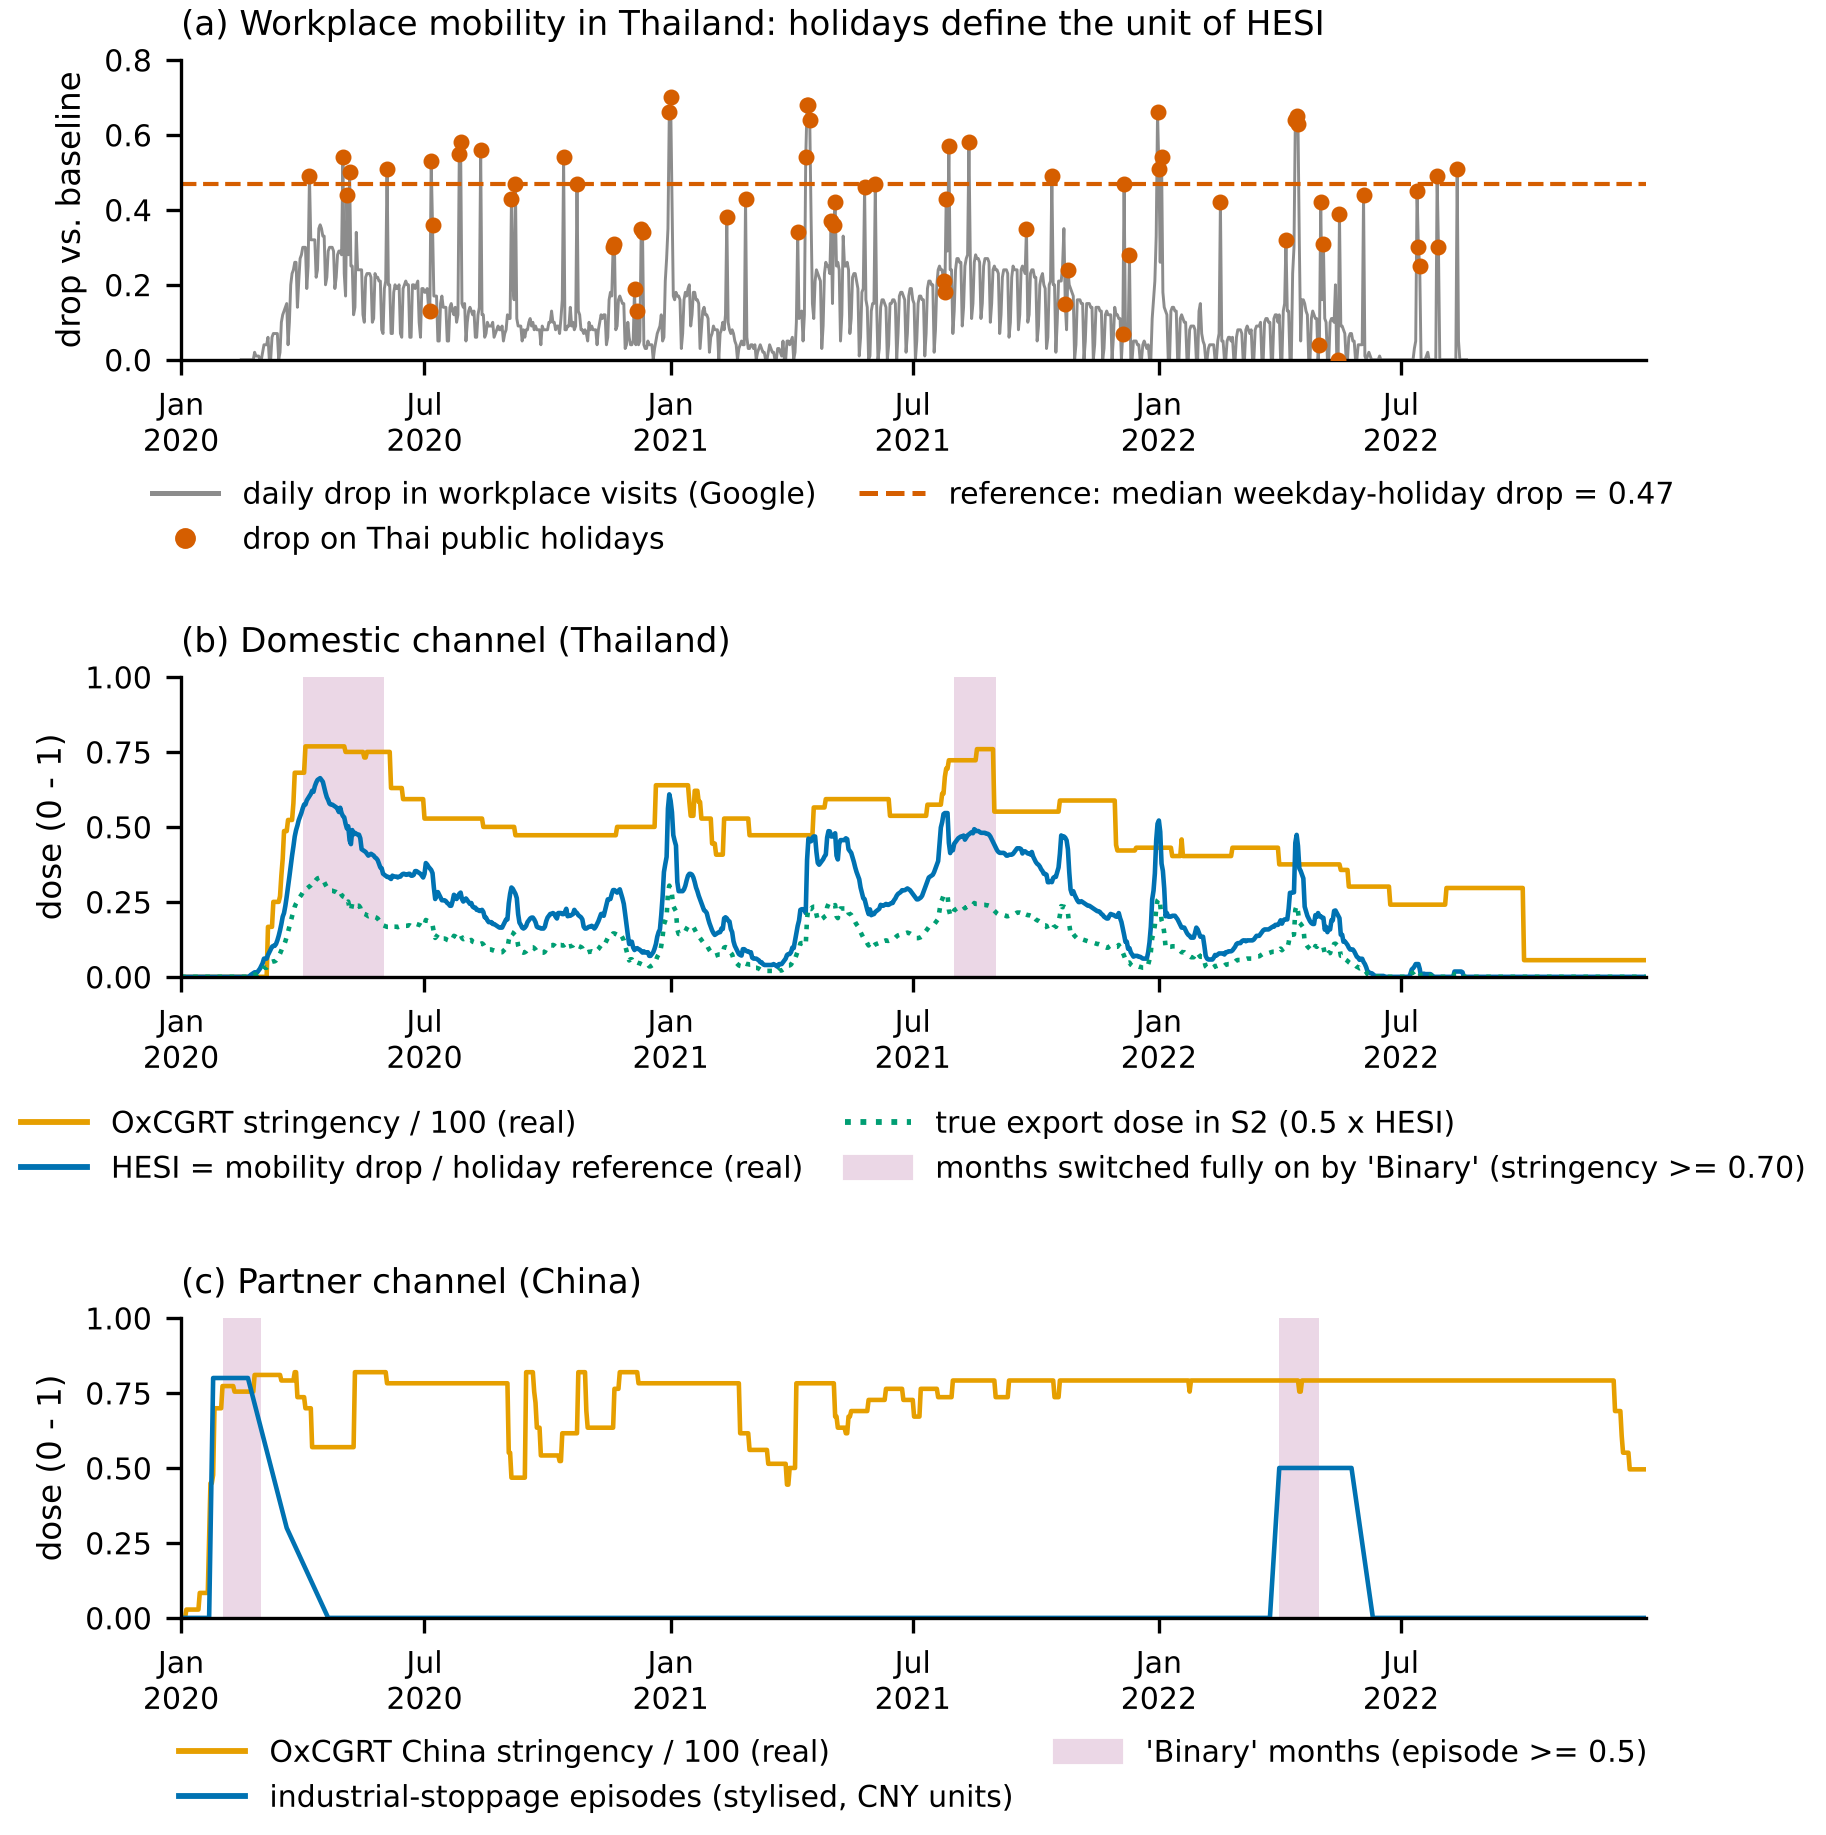
\includegraphics[width=\linewidth]{fig_drivers.png}
\caption{ตัวขับเคลื่อนช่วงโควิดจากข้อมูลจริง (a)~การลดลงของการเดินทางไปที่ทำงานรายวัน จุดสีแดงคือวันหยุดราชการ เส้นประคือค่าอ้างอิง (b)~ช่องทางในประเทศ: stringency ของ OxCGRT, HESI และปริมาณจริงในสถานการณ์ S2 แถบสีม่วงคือเดือนที่ Binary เปิดผลวันหยุดทั้งเดือน (c)~ช่องทางคู่ค้า: stringency ของจีนสูงต่อเนื่องสามปี ขณะที่การหยุดอุตสาหกรรมเกิดเป็นช่วงสั้น ๆ}
\label{fig:drivers}
\end{figure}

\subsection{กระบวนการสร้างข้อมูลจำลอง}
เนื่องจากต้องการทราบค่าจริงของทุกพารามิเตอร์ เราสร้างมูลค่าส่งออกรายวันตั้งแต่ 1 ม.ค. 2010 ถึง 31 ธ.ค. 2024 จากสมการ~\eqref{eq:daily} โดยใช้ตัวขับเคลื่อนจริงข้างต้น ตารางที่~\ref{tab:dgp} สรุปพารามิเตอร์ ระดับและแนวโน้มปรับให้ยอดส่งออกต่อปีอยู่ในหลักสองแสนล้านดอลลาร์สหรัฐเช่นเดียวกับไทย ปริมาณจริงของการหยุดงานมีความคลาดเคลื่อนเชิงสัดส่วน $\nu_d$ ที่เปลี่ยนช้า เพื่อให้ mobility เป็นตัวแทนที่ไม่สมบูรณ์แม้ในสถานการณ์ที่ดีที่สุด เราศึกษาสองสถานการณ์ คือ S1 ซึ่งการถ่ายโอนสมบูรณ์ ($\kappa=1$ ไม่มีช็อกด้านอุปสงค์) และ S2 ซึ่งสมจริงกว่า ($\kappa=0.5$ พร้อมช็อกด้านอุปสงค์ของโลกที่ HESI ไม่รู้จัก) แต่ละรอบใช้ตัวเลขสุ่มชุดเดียวกันในทั้งสองสถานการณ์ (common random numbers) และทำซ้ำ 30 รอบ รูปที่~\ref{fig:data} แสดงตัวอย่างข้อมูล

\begin{table}[t]
\centering\small
\caption{พารามิเตอร์ของกระบวนการสร้างข้อมูลจำลองรายวัน (สเกล log)}
\label{tab:dgp}
\begin{tabular}{p{0.27\linewidth}p{0.66\linewidth}}
\toprule
องค์ประกอบ & ค่าที่ใช้ \\
\midrule
ระดับเริ่มต้น & 560 ล้านดอลลาร์ต่อวันในปี 2010 (ราว 2 แสนล้านดอลลาร์ต่อปี) \\
แนวโน้ม & $+10$\%/ปี (2010--11), $-1$\%/ปี (2012--15), $+2.5$\%/ปี (2016--19), $+3$\%/ปี (2020--22), $+2$\%/ปี (2023--24) \\
ฤดูกาลรายปี & ฟูเรียร์ 3 ฮาร์มอนิก แอมพลิจูดราว $\pm 6$\% \\
วันในสัปดาห์ & จันทร์--ศุกร์ $+0.02$ ถึง $+0.04$, เสาร์ $-0.30$, อาทิตย์ $-0.55$ \\
วันหยุดไทย $\beta_D$ & $\log 0.45=-0.80$ (ยอดหายราว 55\% ในวันหยุด) \\
ตรุษจีน $\beta_P$ & $\log 0.80=-0.22$ ต่อวันในหน้าต่าง $-1\ldots+6$ วัน \\
ปริมาณโควิดจริง & ในประเทศ $\kappa h_d(1+\nu_d)$, คู่ค้า $p_d(1+\nu'_d)$; $\nu$ เป็น AR(1) $\rho=0.97$ ส่วนเบี่ยงเบนคงที่ 0.15 \\
ความคลาดเคลื่อน & AR(1) รายวัน $\rho=0.985$ (ส่วนเบี่ยงเบนคงที่ 0.046), AR(1) รายเดือน $\rho=0.85$ (นวัตกรรม 0.015), iid 0.12 \\
S1 (ถ่ายโอนสมบูรณ์) & $\kappa=1$ ไม่มีช็อกด้านอุปสงค์ \\
S2 (สมจริง) & $\kappa=0.5$; อุปสงค์ $-8$\% ช่วง เม.ย.--มิ.ย. 2020 แล้วฟื้นเป็น $+7$\% ในปี 2021 และจางหายกลางปี 2022 \\
\bottomrule
\end{tabular}
\end{table}

\begin{figure}[t]
\centering
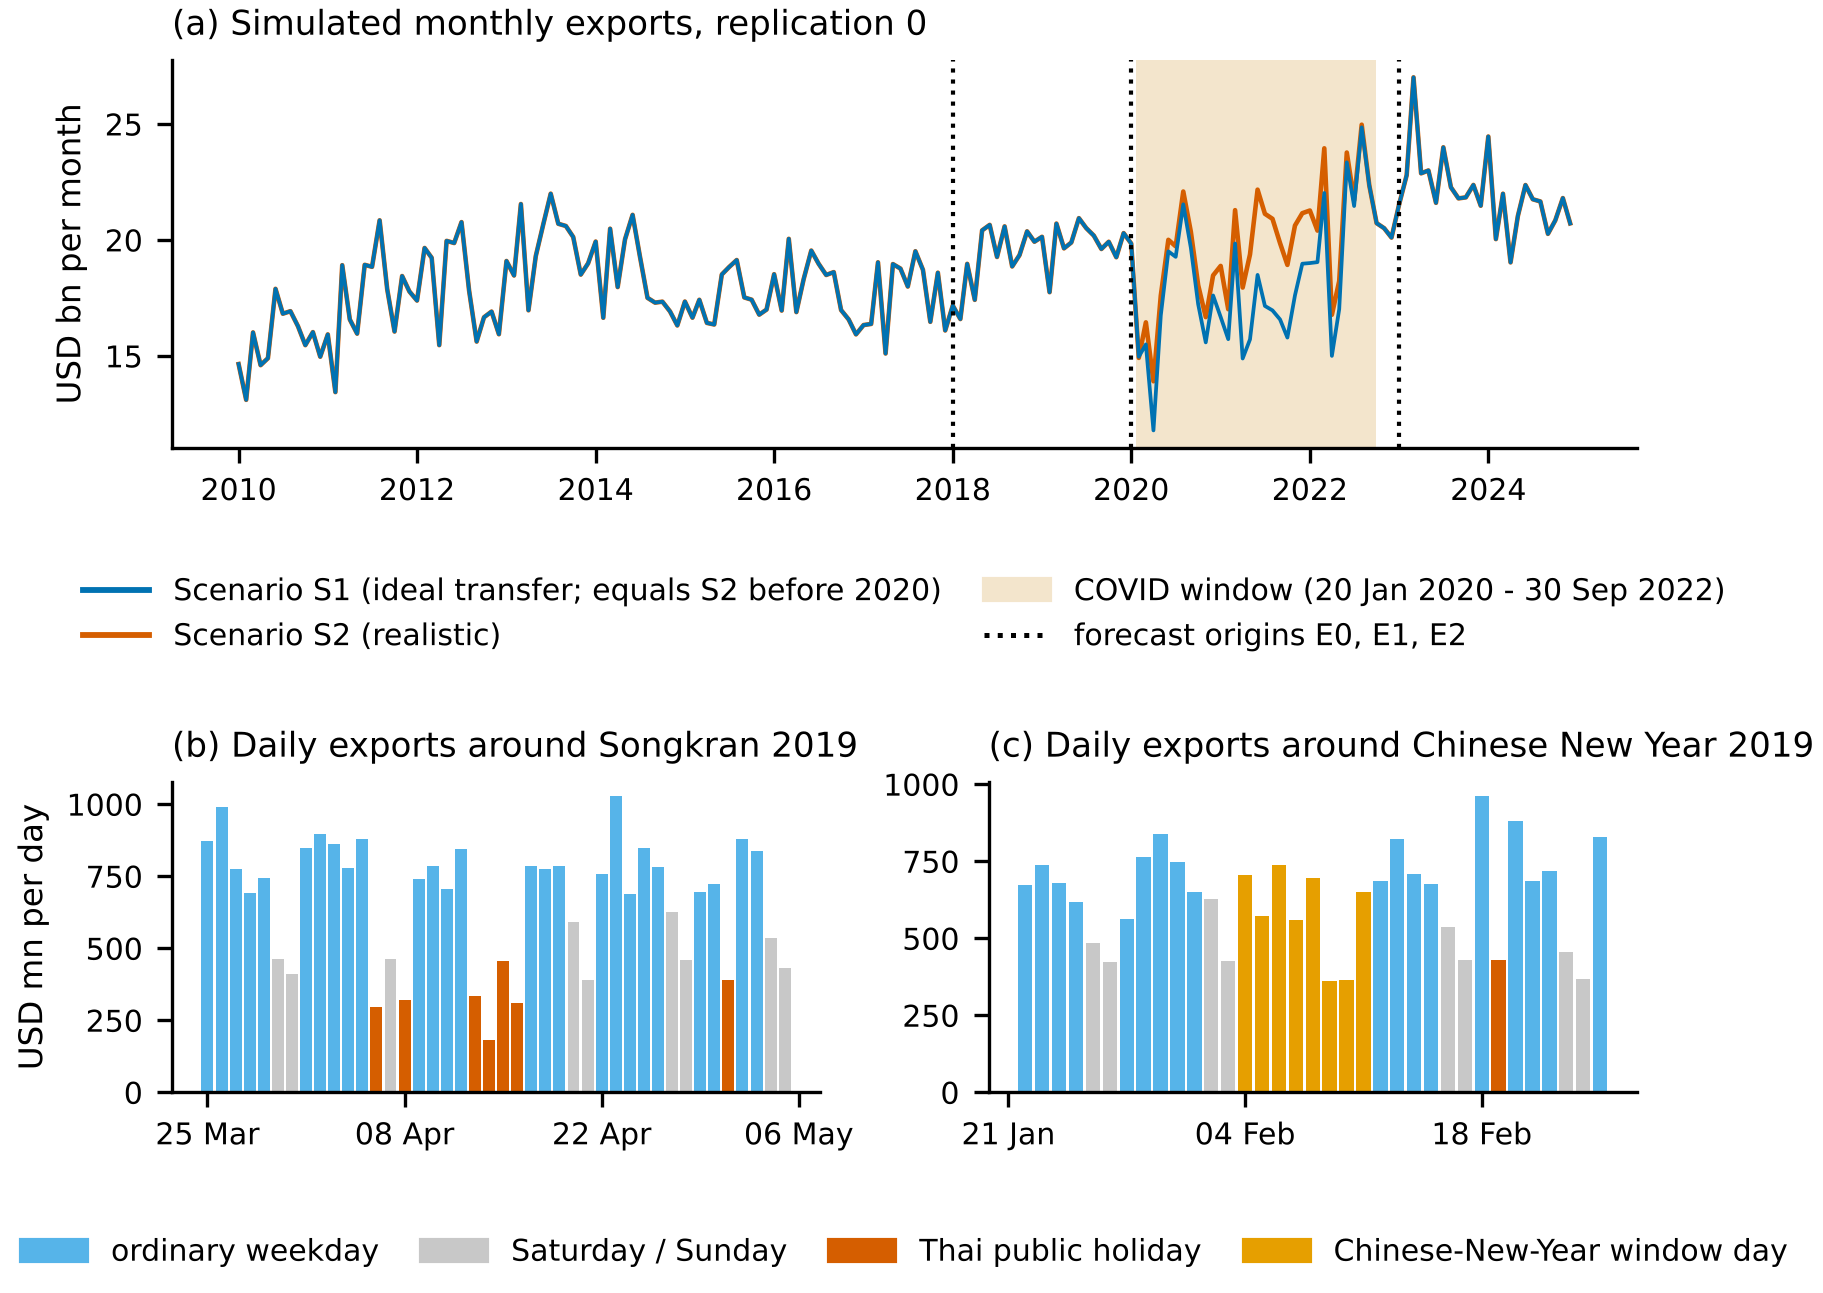
\includegraphics[width=\linewidth]{fig_data.png}
\caption{(a)~มูลค่าส่งออกรายเดือนจำลอง (รอบที่ 0) ของสองสถานการณ์ เส้นจุดคือจุดเริ่มพยากรณ์ของการทดลอง E0, E1 และ E2 (b)--(c)~ข้อมูลรายวันรอบสงกรานต์และตรุษจีนปี 2019 แท่งสีแดงคือวันหยุด แท่งต่ำที่เกิดเป็นจังหวะคือวันเสาร์--อาทิตย์}
\label{fig:data}
\end{figure}

\subsection{แบบจำลอง ตัวแปรเปรียบเทียบ และการทดลอง}
ตารางที่~\ref{tab:models} สรุปแบบจำลองและตัวแปรเปรียบเทียบ ทุกแบบจำลองใช้ hyperparameter ที่กำหนดล่วงหน้า ไม่มีการปรับจูนด้วยข้อมูลทดสอบ การทดลองมีสามชุด
\begin{itemize}
\item \textbf{E0 ช่วงปกติ:} ฝึกถึง ธ.ค. 2017 พยากรณ์ ม.ค. 2018--ธ.ค. 2019
\item \textbf{E1 ช่วงช็อก:} ฝึกถึง ธ.ค. 2019 พยากรณ์ ม.ค. 2020--ธ.ค. 2021 โดยแบบจำลองได้รับตัวขับเคลื่อนที่สังเกตได้ในช่วงพยากรณ์ จึงเป็นการพยากรณ์แบบมีเงื่อนไข (scenario-conditional) หรือ nowcasting ไม่ใช่ ex-ante ประเมินสองหน้าต่าง คือ 24 เดือนเต็ม และ พ.ค. 2020--ธ.ค. 2021 (20 เดือน) ซึ่งเป็นช่วงหลังการปรับเทียบของ HESI-cal
\item \textbf{E2 หลังช็อก:} ฝึกถึง ธ.ค. 2022 (รวมช่วงโควิด) พยากรณ์ ม.ค. 2023--ธ.ค. 2024 โดยไม่มีโควิดในอนาคต
\end{itemize}
ตัวชี้วัดหลักคือ MAPE ของยอดรายเดือน และรายงาน MASE ซึ่งใช้ seasonal naive ในข้อมูลฝึกเป็นตัวหาร ค่าในตารางคือค่าเฉลี่ยจาก 30 รอบ ตัวเลขในวงเล็บคือ standard error

\begin{table}[t]
\centering\small
\caption{แบบจำลองและตัวแปรเปรียบเทียบ}
\label{tab:models}
\begin{tabular}{p{0.24\linewidth}p{0.69\linewidth}}
\toprule
แบบจำลอง & รายละเอียด \\
\midrule
SNaive & ค่าของเดือนเดียวกันในปีล่าสุดของข้อมูลฝึก \\
Prophet-D (vanilla) & Prophet รายวันบน $\log y_d$ (yearly order 10, weekly order 3) ไม่มีตัวแปรปฏิทิน แล้วรวมเป็นรายเดือน \\
Prophet-D HE & Prophet รายวัน + ตัวแปรร่วม $x^D_d, x^P_d$ \\
Prophet-M HE & Prophet รายเดือนบน $\log(Y_m/D_m)$ (yearly order 5, 15 changepoints) + $\bar x^D_m,\bar x^P_m,\mathrm{WK}_m$ \\
Prophet-M HE+AC & Prophet-M HE + aggregation correction (บทแทรก~\ref{cor:ac}) \\
SARIMAX HE & airline $(0,1,1)(0,1,1)_{12}$ บน $\log(Y_m/D_m)$ + ตัวแปรภายนอกชุดเดียวกับ Prophet-M \\
LightGBM-D/M HE & แนวโน้มเชิงเส้น (OLS บน log) + LightGBM บนส่วนเหลือ; รายวันใช้วันในสัปดาห์ วันในปี $x^D, x^P$; รายเดือนใช้เดือน $\bar x^D,\bar x^P,\mathrm{WK}$ \\
\midrule
\multicolumn{2}{l}{\textit{ปริมาณโควิดในช่วงพยากรณ์ (E1)}} \\
Off & ไม่ใส่โควิด ใช้เฉพาะวันหยุด \\
Binary & $x^D=1$ ทั้งเดือนเมื่อ stringency เฉลี่ยของเดือน $\ge 0.70$ และ $x^P=1$ ทั้งเดือนเมื่อ episode จีน $\ge 0.5$ \\
Stringency & ใช้ OxCGRT/100 ของไทยและจีนเป็นปริมาณโดยตรง \\
HESI & $\lambda=1$ บน HESI จาก mobility; ช่องทางคู่ค้าใช้ episode \\
HESI-cal & เลือก $\hat\lambda\in\{0,0.05,\ldots,3\}$ ให้ error ต่ำสุดใน มี.ค.--เม.ย. 2020 แล้วประเมิน พ.ค. 2020--ธ.ค. 2021 \\
Oracle & รู้ค่า $\kappa$ จริง แต่ไม่รู้ $\nu_d$ และช็อกด้านอุปสงค์ \\
\midrule
\multicolumn{2}{l}{\textit{การจัดการช่วงโควิดในข้อมูลฝึก (E2)}} \\
cal / mask / sep & ไม่จัดการ / ตัดช่วง 20 ม.ค. 2020--30 ก.ย. 2022 ออก / ใส่ HESI และ episode เป็นตัวแปรแยกที่มีสัมประสิทธิ์ของตัวเอง \\
binary / stringency / hesi & ใช้ตัวแปรร่วมตามนิยามข้างต้นในข้อมูลฝึก \\
\bottomrule
\end{tabular}
\end{table}

\section{ผลการทดลอง}
\subsection{ช่วงช็อก: การถ่ายโอนได้ผลเมื่อปริมาณถูกต้อง}
ตารางที่~\ref{tab:e1} และรูปที่~\ref{fig:paths} สรุปผลของ E1 ในสถานการณ์ S1 Prophet รายวันที่ใช้ HESI ลด MAPE ช่วงปี 2020--2021 จาก 26.0\% (ไม่ใส่โควิด) เหลือ 7.8\% และดีกว่ากรณีไม่ใส่โควิดใน 100\% ของรอบการจำลอง สิ่งที่ควรสังเกตคือแบบจำลองไม่เคยเห็นข้อมูลโควิดแม้แต่วันเดียว ผลทั้งหมดมาจาก $\hat\beta_D$ ที่เรียนจากวันหยุดก่อนปี 2020

ในทางกลับกัน การเปิดผลวันหยุดทั้งเดือน (Binary) ลด error ได้เพียงเล็กน้อยเหลือ 22.7\% เพราะเลือกเปิดเพียงสามเดือนที่ล็อกดาวน์หนักที่สุด ในเดือนเหล่านั้นค่าพยากรณ์ตกลงมากเกินจริง (ยอดหายราว 55\% ทั้งเดือน) ขณะที่อีกกว่ายี่สิบเดือนที่ได้รับผลกระทบบางส่วนไม่ถูกปรับเลย ส่วนดัชนี stringency ดิบทำให้ error เพิ่มเป็น 27.2\% เพราะช่องทางคู่ค้าได้รับปริมาณ 0.6--0.8 ต่อเนื่องตามดัชนีของจีน

ใน S2 ซึ่งปริมาณจริงเป็นเพียงครึ่งหนึ่งของที่ mobility บอก และมีช็อกด้านอุปสงค์ HESI ($\lambda=1$) ยังดีกว่ากรณีไม่ใส่โควิด (10.9\% เทียบกับ 14.7\%) แต่ยังห่างจาก oracle (8.3\%) เมื่อปรับเทียบ $\lambda$ จากสองเดือนแรก error ในช่วง พ.ค. 2020--ธ.ค. 2021 ลดเหลือ 8.8\% เทียบกับ 13.0\% เมื่อไม่ใส่โควิด และ 8.6\% ของ oracle

ข้อสังเกตที่ต้องระวังคือ ใน S2 แบบจำลองรายเดือนที่ใช้ HESI ($\lambda=1$) ให้ผลดีกว่าแบบรายวัน (8.6\% เทียบกับ 10.9\%) ผลนี้ไม่ได้มาจากข้อได้เปรียบของข้อมูลรายเดือน แต่เกิดจากความผิดพลาดสองชั้นที่หักล้างกันโดยบังเอิญ คือค่าสัมประสิทธิ์รายเดือนถูกลดทอน (หัวข้อ~5.3) ขณะที่ปริมาณจาก mobility สูงเกินจริงสองเท่า เมื่อปริมาณถูกต้อง (S1) ลำดับกลับเป็นแบบรายวันดีกว่า (7.8\% เทียบกับ 11.0\%)

\begin{figure}[t]
\centering
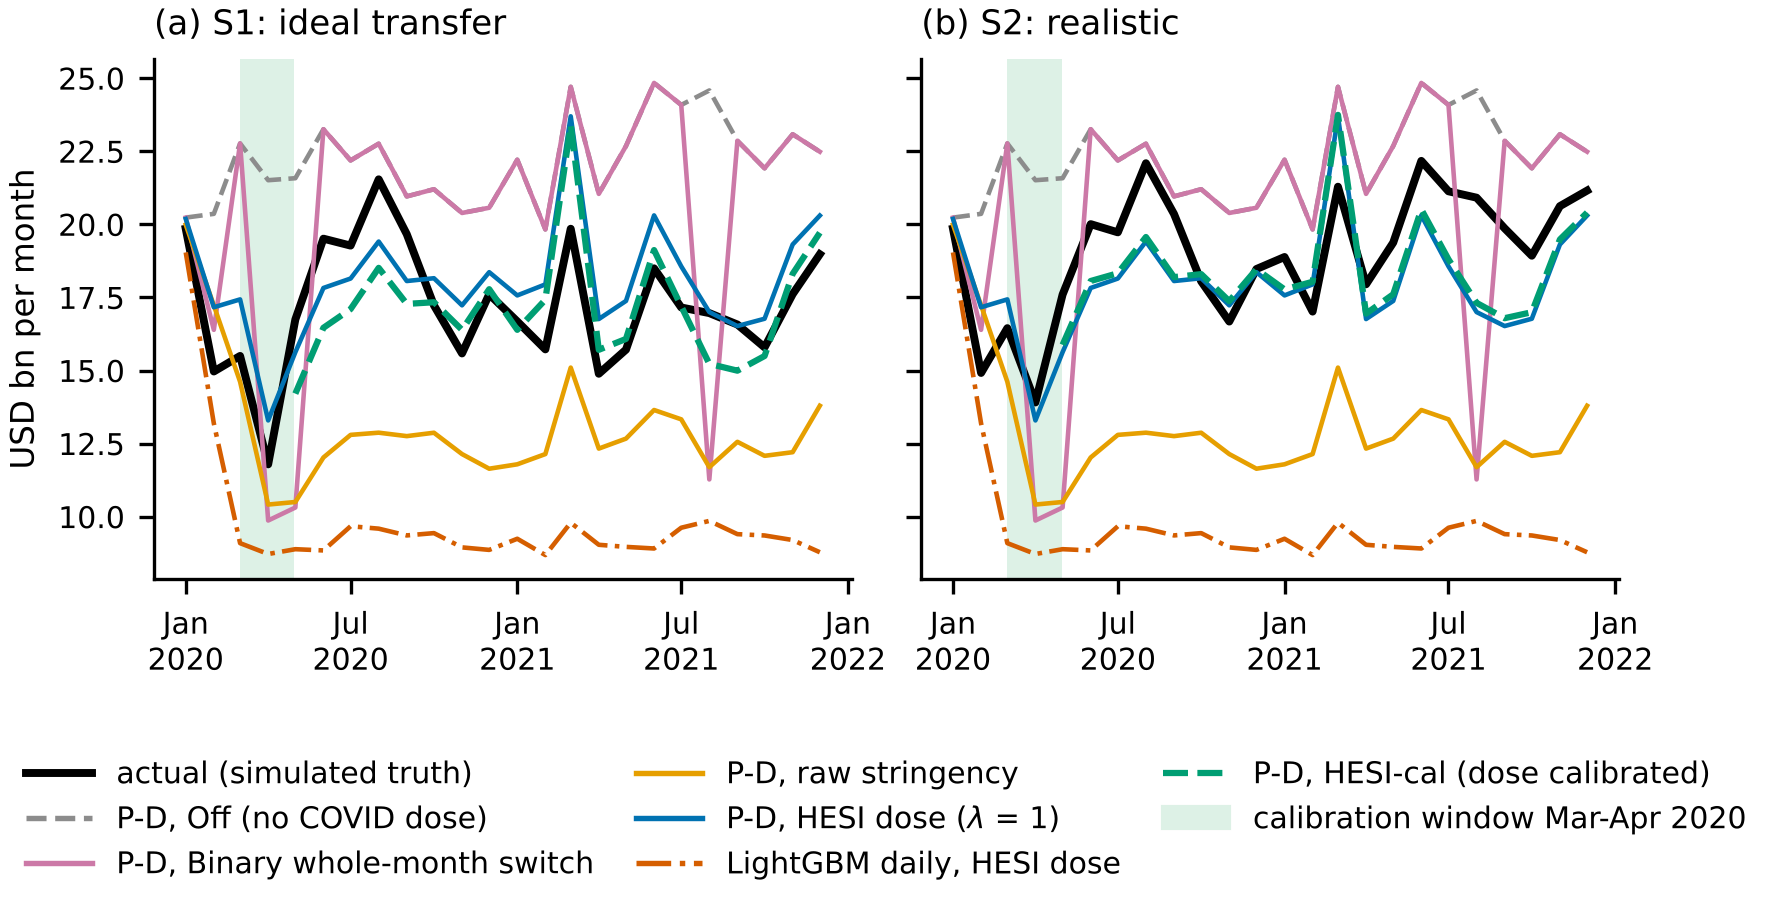
\includegraphics[width=\linewidth]{fig_e1_paths.png}
\caption{ตัวอย่างการพยากรณ์ช่วงช็อก (E1 รอบที่ 0) จากข้อมูลถึงธันวาคม 2019 แถบสีเขียวอ่อนคือสองเดือนที่ใช้ปรับเทียบ HESI-cal}
\label{fig:paths}
\end{figure}

\begin{table}[!tb]
\centering
\caption{ผลช่วงช็อก (E1): MAPE (\%) เฉลี่ยจาก 30 รอบ (standard error) ตัวหนาคือค่าต่ำสุดของแต่ละคอลัมน์ไม่นับ oracle}
\label{tab:e1}
\footnotesize
\begin{tabular}{llcccc}
\toprule
 & & \multicolumn{2}{c}{S1: ถ่ายโอนสมบูรณ์} & \multicolumn{2}{c}{S2: สมจริง} \\
\cmidrule(lr){3-4}\cmidrule(lr){5-6}
แบบจำลอง & ปริมาณโควิด & ม.ค.20--ธ.ค.21 & พ.ค.20--ธ.ค.21 & ม.ค.20--ธ.ค.21 & พ.ค.20--ธ.ค.21 \\
\midrule
SNaive & -- & 20.5 (0.7) & 19.8 (0.8) & 11.1 (0.5) & 9.9 (0.5) \\
\midrule
Prophet-D & Vanilla (ไม่มีปฏิทิน) & 26.4 (1.3) & 26.4 (1.5) & 14.7 (0.9) & 13.8 (1.0) \\
\midrule
Prophet-D HE & Off (ไม่ใส่โควิด) & 26.0 (1.5) & 24.9 (1.7) & 14.7 (1.0) & 13.0 (1.1) \\
 & Binary ทั้งเดือน & 22.7 (1.2) & 23.9 (1.4) & 15.5 (0.7) & 15.0 (0.9) \\
 & Stringency ดิบ & 27.2 (0.9) & 30.5 (1.1) & 34.4 (0.8) & 38.3 (0.9) \\
 & HESI ($\lambda{=}1$) & \textbf{7.8 (0.5)} & 8.1 (0.6) & 10.9 (0.7) & 11.6 (0.8) \\
 & HESI-cal & -- & \textbf{7.7 (0.5)} & -- & 8.8 (0.6) \\
 & Oracle $\kappa$ & 7.8 (0.5) & 8.1 (0.6) & 8.3 (0.5) & 8.6 (0.6) \\
\midrule
Prophet-M HE & Off (ไม่ใส่โควิด) & 26.3 (1.3) & 25.2 (1.5) & 14.5 (0.9) & 12.7 (1.0) \\
 & Binary ทั้งเดือน & 21.2 (1.1) & 22.6 (1.2) & 13.2 (0.6) & 13.1 (0.8) \\
 & Stringency ดิบ & 17.2 (1.1) & 19.2 (1.3) & 24.3 (1.2) & 27.2 (1.4) \\
 & HESI ($\lambda{=}1$) & 11.0 (1.1) & 11.1 (1.2) & 8.6 (0.5) & 9.0 (0.6) \\
 & HESI-cal & -- & 8.9 (0.7) & -- & 9.0 (0.6) \\
 & Oracle $\kappa$ & 11.0 (1.1) & 11.1 (1.2) & 9.3 (0.6) & 9.0 (0.7) \\
\midrule
Prophet-M HE+AC & Binary ทั้งเดือน & 22.8 (1.0) & 23.9 (1.2) & 15.0 (0.7) & 14.4 (0.8) \\
 & Stringency ดิบ & 25.8 (1.8) & 28.8 (2.0) & 32.8 (1.7) & 36.5 (1.8) \\
 & HESI ($\lambda{=}1$) & 9.8 (1.0) & 10.1 (1.1) & 11.3 (0.9) & 12.0 (1.0) \\
 & HESI-cal & -- & 8.0 (0.5) & -- & 8.6 (0.5) \\
 & Oracle $\kappa$ & 9.8 (1.0) & 10.1 (1.1) & 8.9 (0.6) & 9.0 (0.6) \\
\midrule
SARIMAX HE & Off (ไม่ใส่โควิด) & 24.8 (1.2) & 23.7 (1.4) & 13.4 (0.8) & 11.5 (1.0) \\
 & Binary ทั้งเดือน & 19.9 (1.0) & 21.3 (1.2) & 12.3 (0.6) & 12.1 (0.7) \\
 & Stringency ดิบ & 18.1 (1.2) & 20.4 (1.4) & 25.4 (1.3) & 28.6 (1.4) \\
 & HESI ($\lambda{=}1$) & 9.9 (1.0) & 10.0 (1.1) & \textbf{8.5 (0.5)} & 9.1 (0.5) \\
 & HESI-cal & -- & 8.4 (0.7) & -- & 8.6 (0.5) \\
 & Oracle $\kappa$ & 9.9 (1.0) & 10.0 (1.1) & 8.5 (0.6) & 8.3 (0.7) \\
\midrule
LightGBM-D HE & Off (ไม่ใส่โควิด) & 21.7 (0.8) & 20.2 (0.9) & 11.2 (0.5) & 9.1 (0.5) \\
 & Binary ทั้งเดือน & 19.4 (0.5) & 19.9 (0.7) & 12.9 (0.3) & 11.9 (0.4) \\
 & Stringency ดิบ & 40.4 (0.4) & 44.4 (0.5) & 46.2 (0.4) & 50.7 (0.4) \\
 & HESI ($\lambda{=}1$) & 39.7 (0.4) & 43.1 (0.5) & 45.6 (0.4) & 49.5 (0.4) \\
 & HESI-cal & -- & 22.3 (1.5) & -- & 9.1 (0.5) \\
 & Oracle $\kappa$ & 39.7 (0.4) & 43.1 (0.5) & 45.6 (0.4) & 49.5 (0.4) \\
\midrule
LightGBM-M HE & Off (ไม่ใส่โควิด) & 21.6 (0.8) & 19.7 (0.9) & 11.5 (0.5) & 9.1 (0.5) \\
 & Binary ทั้งเดือน & 20.0 (0.7) & 18.5 (0.8) & 10.3 (0.4) & 8.3 (0.4) \\
 & Stringency ดิบ & 15.5 (0.7) & 14.3 (0.7) & 8.9 (0.3) & \textbf{7.8 (0.3)} \\
 & HESI ($\lambda{=}1$) & 16.6 (0.7) & 15.5 (0.8) & 9.2 (0.3) & 8.0 (0.3) \\
 & HESI-cal & -- & 15.8 (0.8) & -- & 8.4 (0.3) \\
 & Oracle $\kappa$ & 16.6 (0.7) & 15.5 (0.8) & 9.3 (0.3) & 8.1 (0.3) \\
\bottomrule
\end{tabular}
\end{table}

\subsection{ความไวต่อปริมาณ}
รูปที่~\ref{fig:lambda} แสดง MAPE เฉลี่ยเมื่อเปลี่ยนตัวคูณ $\lambda$ สำหรับ Prophet รายวัน กราฟเป็นรูปตัว U ที่มีจุดต่ำสุดที่ $\lambda=1.05$ ใน S1 (ค่าจริง 1.0) และ $\lambda=0.60$ ใน S2 (ค่าจริง 0.5) ตรงตามข้อเสนอ~\ref{prop:transfer} แบบจำลองรายเดือนมีจุดต่ำสุดเลื่อนไปทางขวา ($1.55$ สำหรับ Prophet-M และ $1.45$ สำหรับ SARIMAX ใน S1) แปลว่าต้องใช้ปริมาณสูงเกินจริงเพื่อชดเชยค่าสัมประสิทธิ์ที่ถูกลดทอน การแก้อคติ AC ดึงจุดต่ำสุดกลับมาที่ $1.05$ ใน S1 และ $0.55$ ใน S2 ซึ่งใกล้ค่าจริง แต่ความแกว่งของ $\hat\beta$ ทำให้ระดับ error ต่ำสุดยังสูงกว่า Prophet รายวัน

ตารางที่~\ref{tab:lamhat} แสดงค่า $\hat\lambda$ จากการปรับเทียบด้วยสองเดือนแรก Prophet รายวันได้ $1.07$ ใน S1 (ค่าจริง 1) และ $0.72$ ใน S2 (ค่าจริง 0.5) ค่าใน S2 สูงกว่าค่าจริงเพราะช็อกด้านอุปสงค์ในเดือนมีนาคม--เมษายน 2020 ถูกนับรวมเป็นการหยุดงาน ซึ่งเป็นข้อจำกัดที่หลีกเลี่ยงไม่ได้เมื่อปรับเทียบจากยอดส่งออกเพียงอย่างเดียว

\begin{figure}[t]
\centering
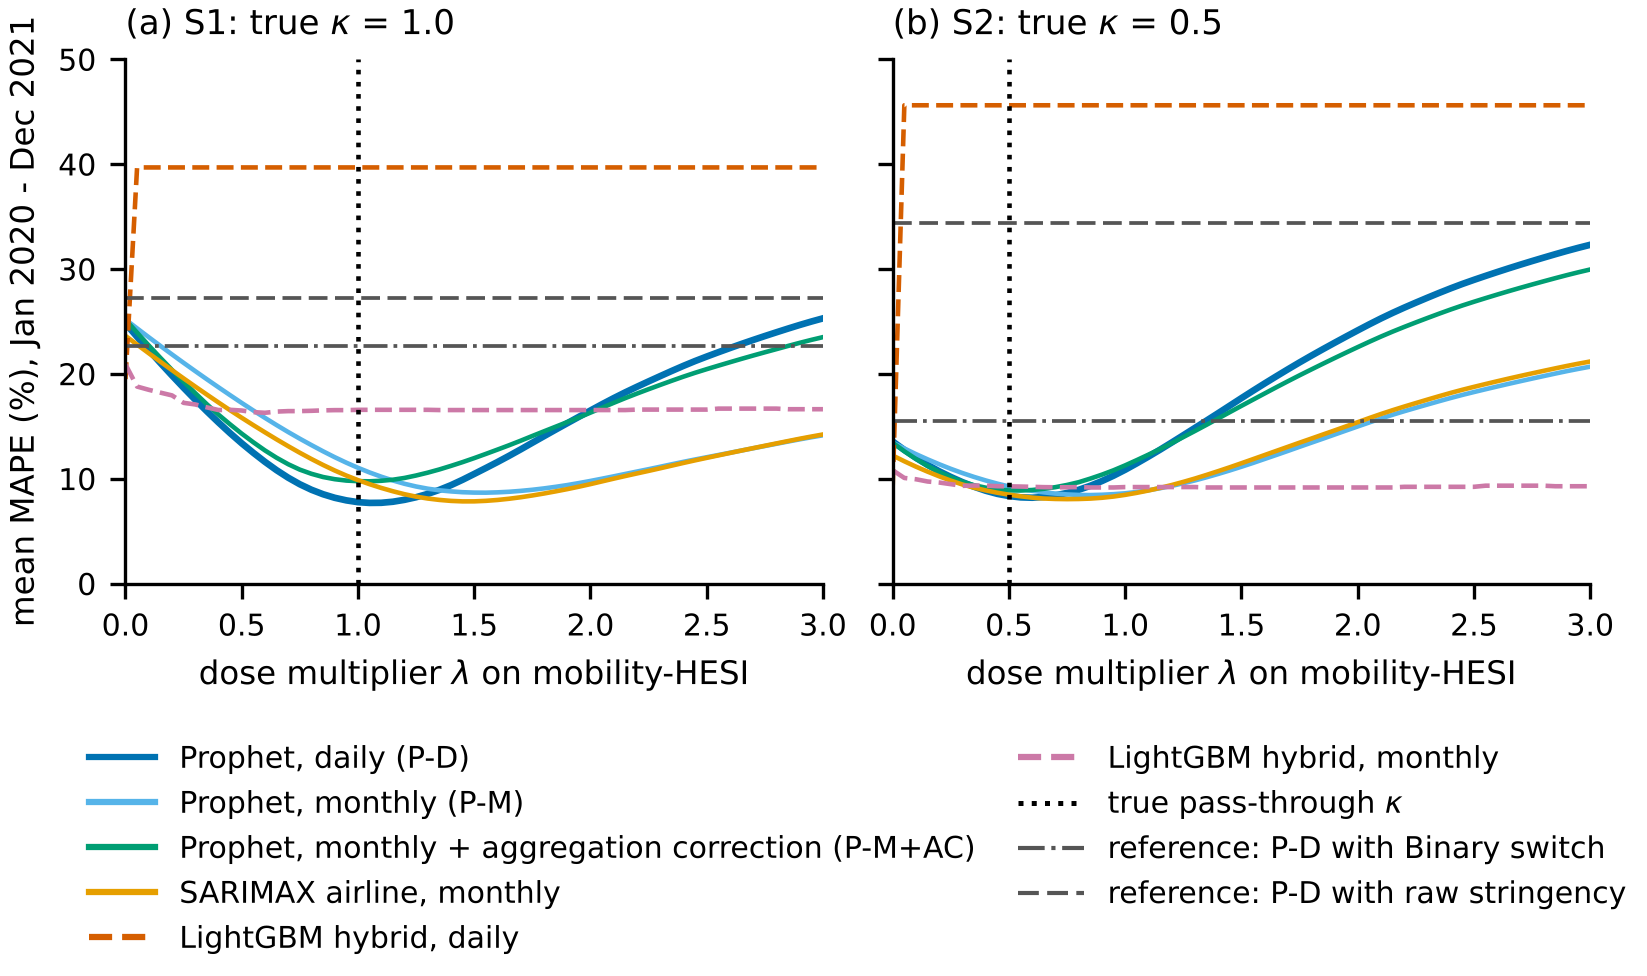
\includegraphics[width=\linewidth]{fig_lambda.png}
\caption{MAPE เฉลี่ยช่วงปี 2020--2021 ตามตัวคูณปริมาณ $\lambda$ เส้นจุดแนวตั้งคือค่าจริง $\kappa$ เส้นแนวนอนคือ Prophet รายวันแบบ Binary และ Stringency LightGBM รายวันกระโดดขึ้นทันทีที่ $\lambda>0$}
\label{fig:lambda}
\end{figure}

\begin{table}[t]
\centering\small
\caption{ค่า $\hat\lambda$ จากการปรับเทียบด้วย มี.ค.--เม.ย. 2020 (ค่าเฉลี่ยและส่วนเบี่ยงเบนมาตรฐาน) ค่าจริงคือ 1.0 ใน S1 และ 0.5 ใน S2}
\label{tab:lamhat}
\begin{tabular}{lcccc}
\toprule
 & \multicolumn{2}{c}{S1} & \multicolumn{2}{c}{S2} \\
\cmidrule(lr){2-3}\cmidrule(lr){4-5}
แบบจำลอง & เฉลี่ย & SD & เฉลี่ย & SD \\
\midrule
Prophet-D HE & 1.07 & 0.20 & 0.72 & 0.18 \\
Prophet-M HE & 1.87 & 0.67 & 1.19 & 0.53 \\
Prophet-M HE+AC & 1.24 & 0.51 & 0.83 & 0.35 \\
SARIMAX HE & 1.77 & 0.56 & 1.12 & 0.44 \\
LightGBM-D HE & 0.01 & 0.02 & 0.00 & 0.00 \\
LightGBM-M HE & 0.44 & 0.26 & 0.45 & 0.26 \\
\bottomrule
\end{tabular}
\end{table}

\subsection{ข้อมูลรายวันเทียบกับรายเดือน}
รูปที่~\ref{fig:beta} และตารางที่~\ref{tab:beta} ยืนยันข้อเสนอ~\ref{prop:jensen} และ~\ref{prop:ident} Prophet รายวันประมาณ $\beta_D$ ได้ $-0.80$ (SD $0.01$) เทียบกับค่าจริง $-0.80$ แบบจำลองรายเดือนได้ $-0.54$ (SD $0.13$) และ SARIMAX ได้ $-0.54$ (SD $0.14$) ค่าเฉลี่ยของแบบจำลองรายเดือนใกล้กับค่าที่คาดจากอคติการรวม ($-0.57$) แสดงว่าการลดทอนส่วนใหญ่มาจากอคติการรวม ขณะที่ collinearity กับฤดูกาลเดือนเมษายนทำให้ค่าประมาณแกว่งมากกว่ารายวันกว่าสิบเท่า (SD $0.13$ เทียบกับ $0.01$) AC ให้ค่าเฉลี่ย $-0.76$ ซึ่งใกล้ค่าจริงขึ้น แต่แกว่งมาก (SD $0.27$) สำหรับช่องทางคู่ค้า ตรุษจีนเลื่อนไปมาระหว่างมกราคมและกุมภาพันธ์ แบบจำลองรายเดือนจึงแทบไม่ลดทอน ($-0.20$ เทียบกับ $-0.22$) แต่แกว่งกว่ารายวันมาก (SD $0.09$ เทียบกับ $0.02$) ข้อค้นพบนี้สนับสนุนการใช้ข้อมูลรายวันหากเข้าถึงได้

\begin{figure}[t]
\centering
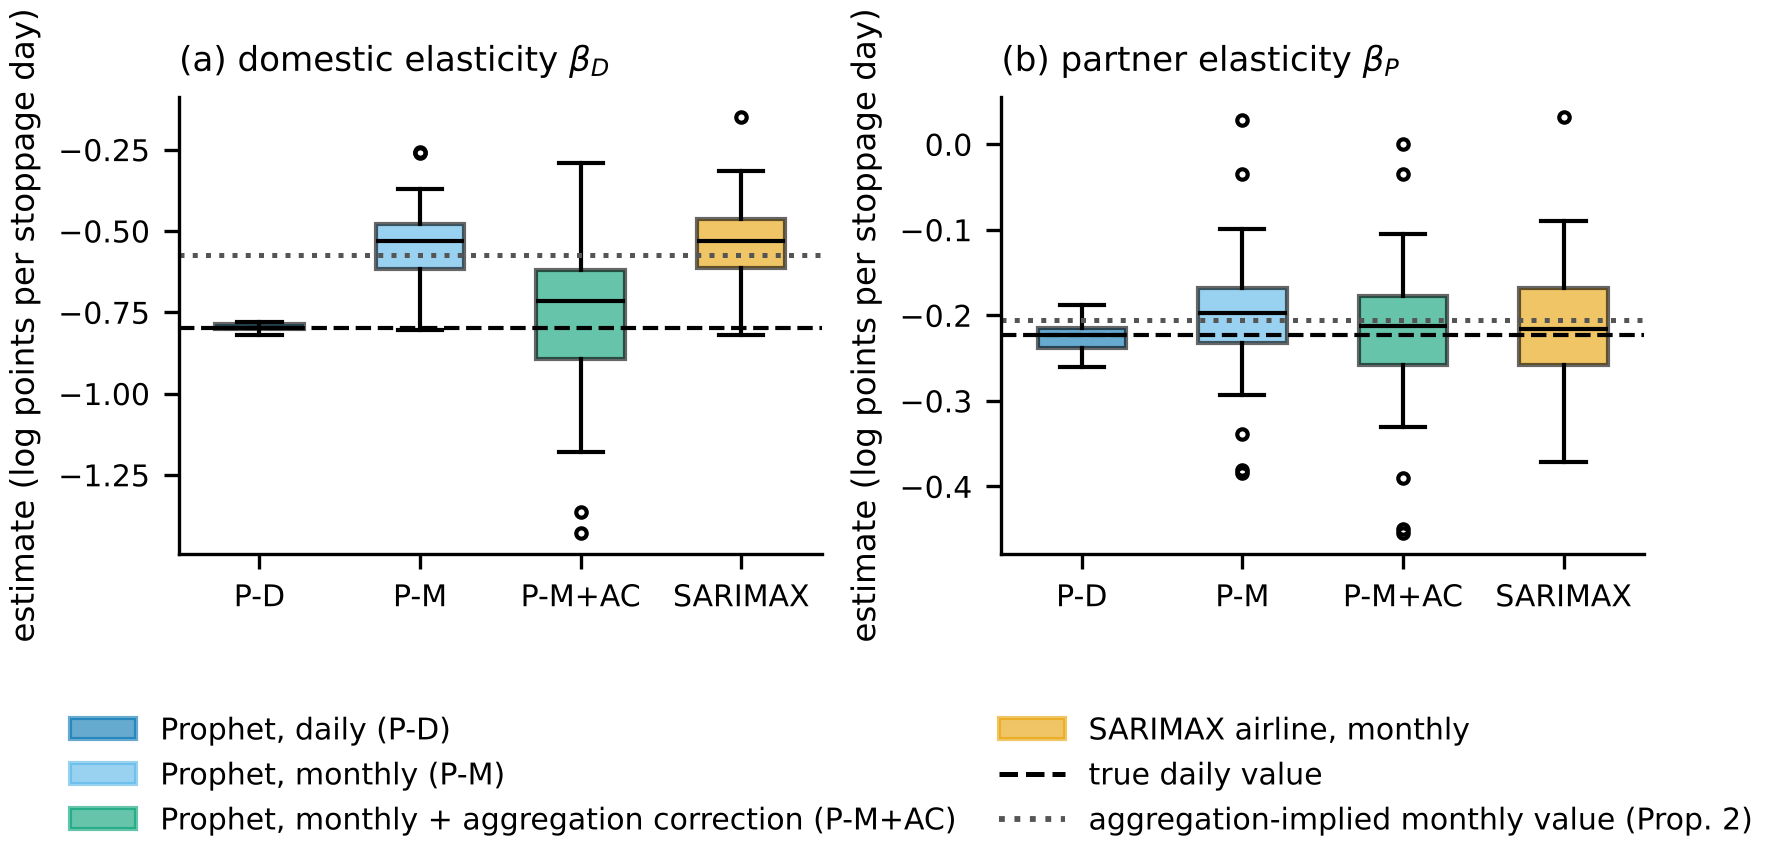
\includegraphics[width=\linewidth]{fig_beta.png}
\caption{การกระจายของค่าสัมประสิทธิ์ที่ประมาณจากข้อมูลก่อนโควิด เส้นประคือค่าจริงรายวัน เส้นจุดคือค่าที่คาดจากการรวมเป็นรายเดือน (ข้อเสนอ~\ref{prop:jensen})}
\label{fig:beta}
\end{figure}

\begin{table}[t]
\centering\small
\caption{ค่าสัมประสิทธิ์ที่ประมาณได้ (E1, ข้อมูลถึง ธ.ค. 2019): ค่าเฉลี่ย ส่วนเบี่ยงเบนมาตรฐาน และ RMSE เทียบค่าจริงรายวัน}
\label{tab:beta}
\begin{tabular}{lcccccc}
\toprule
 & \multicolumn{3}{c}{$\beta_D$ (ในประเทศ)} & \multicolumn{3}{c}{$\beta_P$ (คู่ค้า)} \\
\cmidrule(lr){2-4}\cmidrule(lr){5-7}
วิธี & เฉลี่ย & SD & RMSE & เฉลี่ย & SD & RMSE \\
\midrule
Prophet รายวัน & -0.796 & 0.010 & 0.010 & -0.225 & 0.017 & 0.017 \\
Prophet รายเดือน & -0.540 & 0.131 & 0.289 & -0.203 & 0.086 & 0.086 \\
Prophet รายเดือน + AC & -0.764 & 0.268 & 0.266 & -0.225 & 0.099 & 0.097 \\
SARIMAX รายเดือน & -0.538 & 0.137 & 0.294 & -0.215 & 0.087 & 0.086 \\
\midrule
ค่าจริงรายวัน & -0.799 & & & -0.223 & & \\
ค่าที่คาดจากการรวมเป็นรายเดือน & -0.573 & & & -0.206 & & \\
\bottomrule
\end{tabular}
\end{table}

\subsection{แบบจำลองต้นไม้}
LightGBM รายวันเห็นตัวแปรการหยุดงานเพียงค่า 0 และ 1 ในข้อมูลฝึก และวางจุดตัดที่ $10^{-35}$ ในทุกต้นไม้ (ตรวจจากโครงสร้างต้นไม้ที่ฝึกแล้ว) วันที่มีปริมาณมากกว่าศูนย์แม้เพียงเล็กน้อยจึงถูกมองเป็นวันหยุดเต็มวัน MAPE จึงพุ่งเป็น 39.7\% ใน S1 และ 45.6\% ใน S2 และการปรับเทียบเลือก $\hat\lambda$ ที่ศูนย์หรือใกล้ศูนย์แทบทุกรอบ (ค่าเฉลี่ย $0.01$) LightGBM รายเดือนเห็นค่า $\bar x^D_m$ สูงสุดราว 0.2 ในข้อมูลฝึก แต่เดือนล็อกดาวน์มีค่าถึง 0.6 จึงให้ผลเท่ากับเดือนที่มีวันหยุดมากที่สุดที่เคยเห็น และลด error ได้เพียงจาก 21.6\% เป็น 16.6\% ใน S1 ข้อจำกัดนี้ไม่ได้เกิดจากการปรับ hyperparameter แต่เป็นคุณสมบัติเชิงโครงสร้างของต้นไม้ (ข้อเสนอ~\ref{prop:tree})

\subsection{หลังช็อก: ใครพยากรณ์ปี 2023--2024 ได้ดี}
ตารางที่~\ref{tab:e2} และรูปที่~\ref{fig:e2} แสดงผลของ E2 เมื่อไม่จัดการช่วงโควิด Prophet รายวันได้ MAPE 8.8\% ใน S1 และ 10.8\% ใน S2 การใช้ HESI ในข้อมูลฝึกลดเหลือ 6.2\% และ 8.4\% ส่วนการตัดช่วงโควิดออก (mask) ได้ 6.1\% และ 6.1\% ซึ่งดีเท่ากันหรือดีกว่า โดยเฉพาะใน S2 ที่ปริมาณสูงเกินจริงและช็อกด้านอุปสงค์ที่ไม่ได้อธิบายรั่วเข้าไปในแนวโน้ม SARIMAX ซึ่งปรับระดับตามข้อมูลล่าสุดได้เร็ว ทำผลได้ดีที่สุดโดยรวม (5.7\% และ 5.7\%) ผลที่ชัดที่สุดคือความเสียหายจาก stringency ดิบ (30.4\% และ 34.8\%) เมื่อดัชนีของจีนค้างที่ 0.6--0.8 ตลอดช่วงโควิดในข้อมูลฝึกแล้วกลายเป็นศูนย์ในช่วงพยากรณ์ แบบจำลองจึงคาดว่ายอดส่งออกจะกระโดดขึ้นทันที

\begin{table}[t]
\centering
\caption{ผลหลังช็อก (E2, ม.ค. 2023--ธ.ค. 2024): MAPE (\%) เฉลี่ย (standard error) และ MASE เฉลี่ย}
\label{tab:e2}
\footnotesize
\begin{tabular}{llcccc}
\toprule
 & & \multicolumn{2}{c}{S1} & \multicolumn{2}{c}{S2} \\
\cmidrule(lr){3-4}\cmidrule(lr){5-6}
แบบจำลอง & การจัดการช่วงโควิด & MAPE & MASE & MAPE & MASE \\
\midrule
SNaive & -- & 12.4 (0.4) & 1.57 & 9.5 (0.4) & 1.33 \\
\midrule
Prophet-D & Vanilla (ไม่มีปฏิทิน) & 8.0 (0.3) & 1.00 & 8.9 (0.6) & 1.21 \\
 & Calendar only & 8.8 (0.6) & 1.09 & 10.8 (0.8) & 1.46 \\
 & Mask ช่วงโควิด & 6.1 (0.3) & 0.76 & 6.1 (0.3) & 0.84 \\
 & Separate COVID reg. & 6.3 (0.3) & 0.79 & 9.6 (0.8) & 1.30 \\
 & Binary ทั้งเดือน & 7.1 (0.5) & 0.92 & 6.3 (0.4) & 0.88 \\
 & Stringency ดิบ & 30.4 (1.3) & 3.76 & 34.8 (1.3) & 4.75 \\
 & HESI ($\lambda{=}1$) & 6.2 (0.3) & 0.78 & 8.4 (0.7) & 1.14 \\
\midrule
Prophet-M & Vanilla (ไม่มีปฏิทิน) & 9.4 (0.7) & 1.20 & 7.3 (0.4) & 1.01 \\
 & Calendar only & 8.8 (0.7) & 1.13 & 7.4 (0.5) & 1.02 \\
 & Mask ช่วงโควิด & 6.3 (0.4) & 0.78 & 6.3 (0.4) & 0.87 \\
 & Separate COVID reg. & 6.0 (0.3) & 0.75 & 8.6 (0.7) & 1.16 \\
 & Binary ทั้งเดือน & 9.3 (0.7) & 1.20 & 6.9 (0.4) & 0.95 \\
 & Stringency ดิบ & 23.6 (1.8) & 2.92 & 34.3 (2.0) & 4.66 \\
 & HESI ($\lambda{=}1$) & 6.1 (0.3) & 0.76 & 8.6 (0.7) & 1.16 \\
\midrule
SARIMAX & Calendar only & 6.7 (0.3) & 0.85 & 5.9 (0.3) & 0.82 \\
 & HESI ($\lambda{=}1$) & \textbf{5.7 (0.3)} & 0.71 & \textbf{5.7 (0.3)} & 0.79 \\
\midrule
LightGBM-D & HESI ($\lambda{=}1$) & 13.4 (0.6) & 1.72 & 8.7 (0.5) & 1.26 \\
\midrule
LightGBM-M & HESI ($\lambda{=}1$) & 12.7 (0.6) & 1.64 & 8.4 (0.5) & 1.20 \\
\bottomrule
\end{tabular}
\end{table}

\begin{figure}[t]
\centering
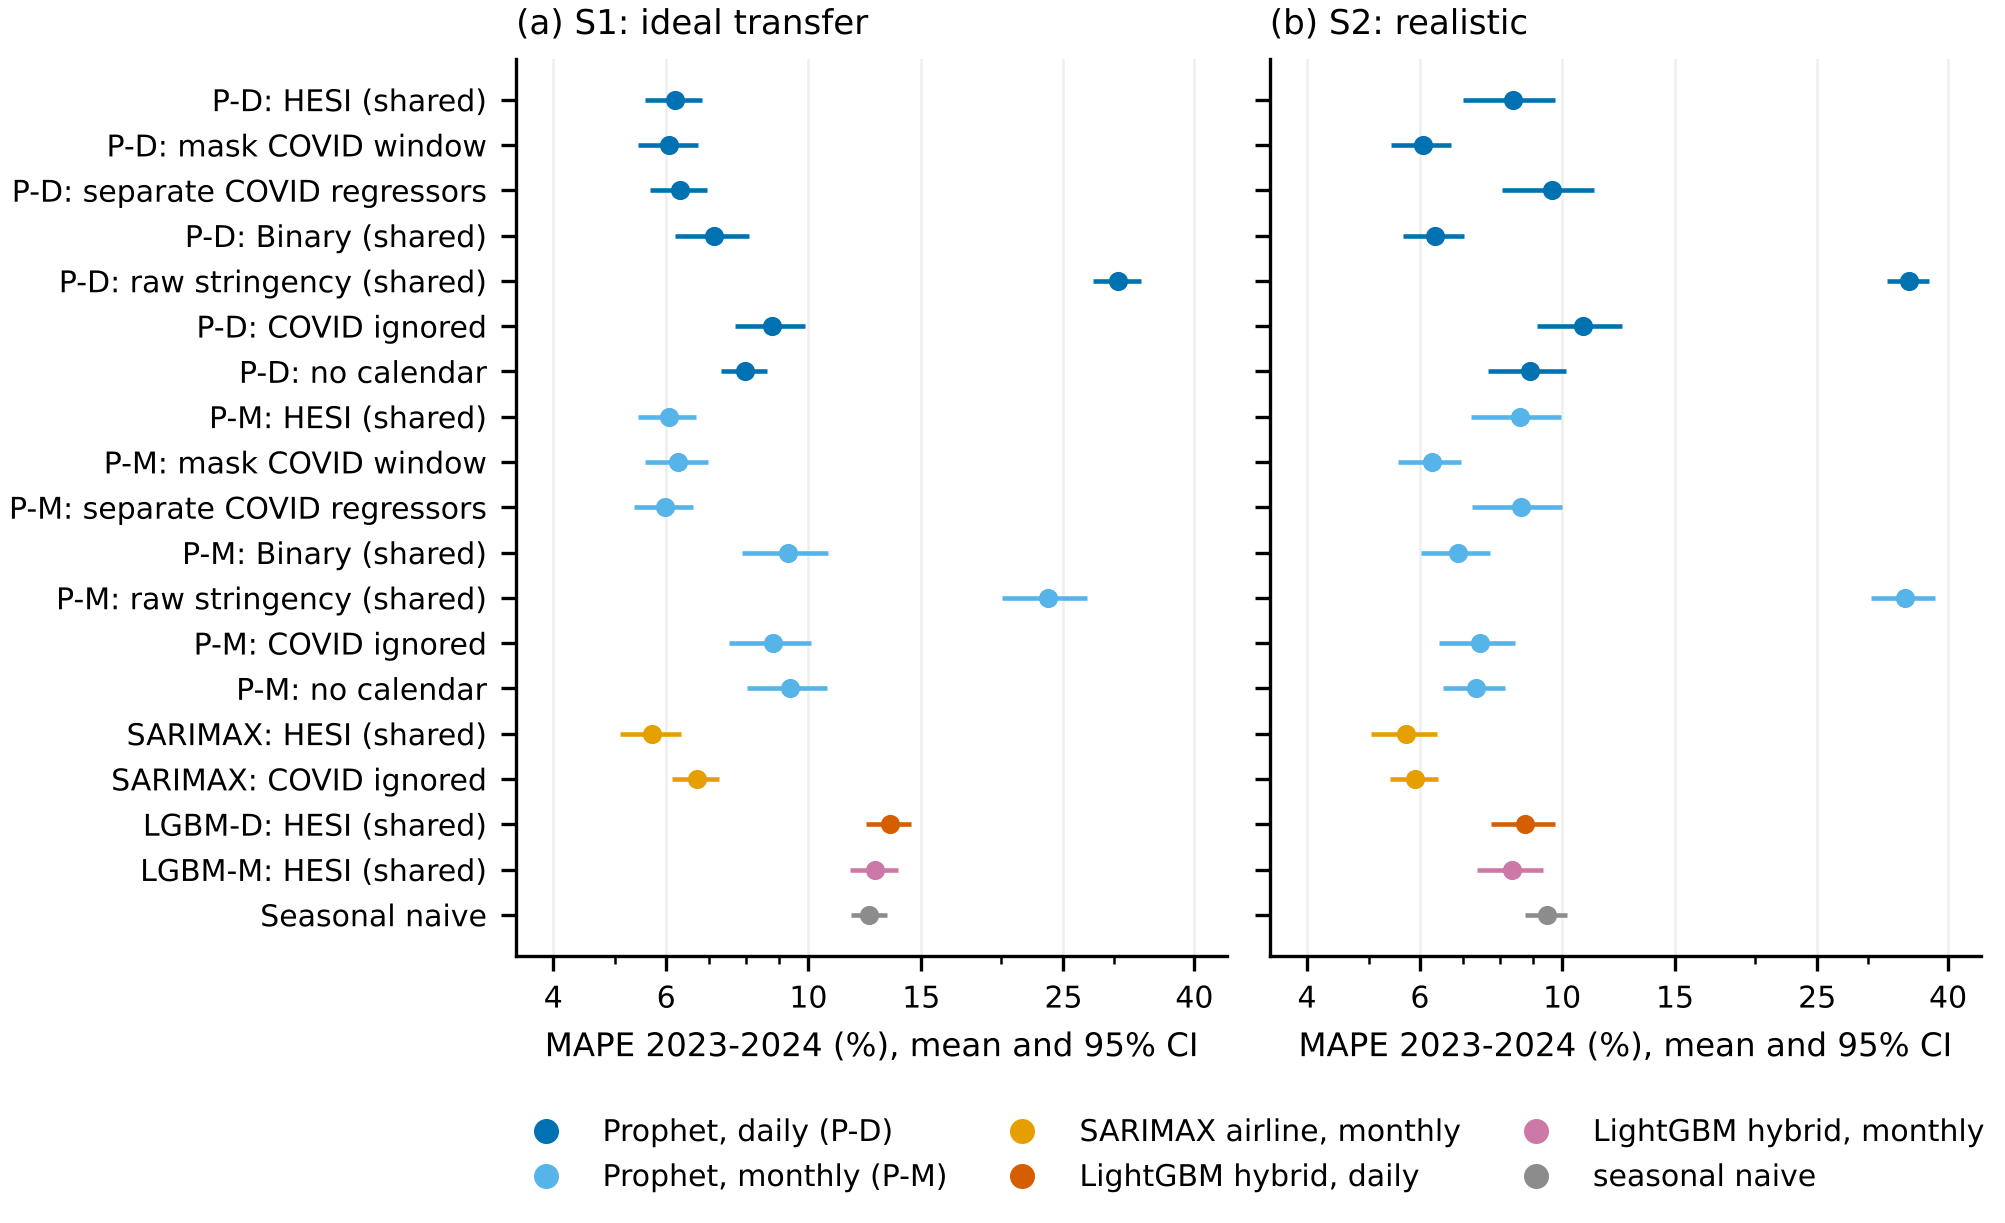
\includegraphics[width=\linewidth]{fig_e2.png}
\caption{MAPE ช่วงหลังช็อก (2023--2024) พร้อมช่วงความเชื่อมั่น 95\% แกนนอนเป็นสเกลลอการิทึม}
\label{fig:e2}
\end{figure}

\subsection{ช่วงปกติ}
ตารางที่~\ref{tab:e0} แสดงว่าในช่วงที่ไม่มีช็อก LightGBM รายวันแม่นที่สุด (4.7\%) ตามด้วย LightGBM รายเดือน (5.5\%) และ SARIMAX (5.9\%) ส่วน Prophet อยู่ราว 7.3\% ใกล้เคียง seasonal naive (7.5\%) และตัวแปรปฏิทินช่วย Prophet รายวันได้เพียงเล็กน้อย (7.4\% เป็น 7.3\%) ผลนี้ย้ำว่าข้อได้เปรียบของ HES อยู่ที่การถ่ายโอนในช่วงช็อก ไม่ใช่ความแม่นยำทั่วไปของ Prophet

\begin{table}[t]
\centering\small
\caption{ผลช่วงปกติ (E0, ม.ค. 2018--ธ.ค. 2019): MAPE (\%) เฉลี่ย (standard error) และ MASE เฉลี่ย}
\label{tab:e0}
\begin{tabular}{llcc}
\toprule
แบบจำลอง & ตัวแปร & MAPE & MASE \\
\midrule
SNaive & -- & 7.5 (0.3) & 1.08 \\
Prophet-D & Vanilla (ไม่มีปฏิทิน) & 7.4 (0.6) & 1.06 \\
Prophet-D HE & ปฏิทิน (holiday regressors) & 7.3 (0.7) & 1.05 \\
Prophet-M & Vanilla (ไม่มีปฏิทิน) & 7.2 (0.6) & 1.03 \\
Prophet-M HE & ปฏิทิน (holiday regressors) & 6.9 (0.6) & 0.99 \\
Prophet-M HE+AC & ปฏิทิน (holiday regressors) & 6.9 (0.6) & 0.99 \\
SARIMAX HE & ปฏิทิน (holiday regressors) & 5.9 (0.4) & 0.85 \\
LightGBM-D HE & ปฏิทิน (holiday regressors) & \textbf{4.7 (0.2)} & 0.67 \\
LightGBM-M HE & ปฏิทิน (holiday regressors) & 5.5 (0.2) & 0.79 \\
\bottomrule
\end{tabular}
\end{table}

\section{อภิปราย}
\subsection{สิ่งที่แนวคิดตั้งต้นถูก และสิ่งที่ต้องปรับ}
แนวคิดตั้งต้นของงานนี้มีสามส่วน ส่วนแรกคือ “ล็อกดาวน์คล้ายวันหยุด จึงเรียนผลจากสงกรานต์และตรุษจีนได้” ผลการจำลองสนับสนุนส่วนนี้อย่างชัดเจน ภายใต้เงื่อนไขว่าใช้ตัวแปรร่วม ไม่ใช่วันหยุดชื่อใหม่ ส่วนที่สองคือ “เปิดผลวันหยุดทั้งเดือนในช่วงโควิด” ส่วนนี้ต้องปรับ เพราะวันล็อกดาวน์ไม่ได้หยุดเท่าวันหยุด การเปิดทั้งเดือนจึงเกินจริงในเดือนที่เลือกและพลาดเดือนอื่นทั้งหมด ทางแก้คือใช้ปริมาณที่วัดได้และปรับเทียบเมื่อมีข้อมูลจริงเข้ามา ส่วนที่สามคือ “ใช้ข้อมูลรายวันจะดีกว่า” ผลสนับสนุนพร้อมเหตุผลเชิงทฤษฎีสองข้อ คือข้อมูลรายวันไม่มีอคติจากการรวม และระบุค่าผลวันหยุดได้โดยไม่ชนกับฤดูกาล ส่วนข้อสงสัยว่าแบบจำลองต้นไม้รับมือเหตุการณ์นี้ไม่ได้ก็ได้รับการยืนยันในช่วงช็อก แต่ในช่วงปกติต้นไม้กลับแม่นที่สุด การใช้แบบจำลองต่างกันตามสภาวะ หรือการให้ต้นไม้เรียนจากส่วนเหลือหลังหักผลการหยุดงานที่ประมาณโดยแบบจำลองเชิงเส้น จึงเป็นแนวทางที่น่าทดลองต่อ

\subsection{ข้อเสนอสำหรับการนำไปใช้กับข้อมูลส่งออกจริง}
\begin{enumerate}
\item ใช้มูลค่าส่งออกรายเดือนแบบไม่รวมทองคำเป็นอนุกรมหลัก และบันทึกวันที่ดาวน์โหลดข้อมูล (vintage)
\item สร้างปฏิทินวันหยุดตามที่หยุดจริง และหน้าต่างตรุษจีน
\item สร้าง HESI จาก Google Mobility โดยพิจารณาแยกค่าอ้างอิงของเทศกาลใหญ่ (สงกรานต์และปีใหม่) ออกจากวันหยุดเดี่ยว และใช้ episode หรือตัวแทนที่ดีกว่าสำหรับจีน ห้ามใช้ stringency ดิบ
\item ถ้ามีข้อมูลรายวัน ใช้ Prophet-D HE ถ้าไม่มี ใช้ Prophet-M HE+AC คู่กับ SARIMAX
\item ปรับเทียบ $\lambda$ ด้วยเดือนที่ประกาศตัวเลขแล้ว และรายงานความไม่แน่นอนของ $\hat\lambda$
\item สำหรับการพยากรณ์หลังช็อก เปรียบเทียบ mask, HESI และ SARIMAX ด้วย rolling origin และทดสอบความต่างด้วย Diebold--Mariano \citep{diebold1995comparing} พร้อมการปรับแก้ของ \citet{harvey1997testing}
\item รายงานผลแบบมีเงื่อนไขแยกจากผลแบบ ex-ante เสมอ
\end{enumerate}

\subsection{ข้อจำกัด}
งานนี้มีข้อจำกัดสำคัญหกข้อ ข้อแรก ผลทั้งหมดมาจากข้อมูลส่งออกจำลอง ขนาดของผลในข้อมูลจริงอาจต่างออกไป ข้อสอง DGP สมมติความสัมพันธ์แบบ log-linear และผลเท่ากันในทุกวันหยุด ขณะที่ข้อมูล mobility จริงชี้ว่าสงกรานต์และปีใหม่หนักกว่าวันหยุดเดี่ยว ข้อสาม mobility วัดการไปที่ทำงาน ไม่ใช่การผลิต และอัตราการส่งผ่าน $\kappa$ อาจเปลี่ยนตามเวลาเมื่อธุรกิจปรับตัว ข้อสี่ ช็อกด้านอุปสงค์ของโลกไม่ใช่การหยุดงาน HESI จึงอธิบายส่วนนี้ไม่ได้ ข้อห้า episode ของจีนเป็นค่าที่กำหนดขึ้นจากเหตุการณ์ ไม่ใช่ข้อมูลวัด และข้อหก E1 เป็นการพยากรณ์แบบมีเงื่อนไขที่ใช้ตัวขับเคลื่อนที่สังเกตได้และค่าเฉลี่ยเคลื่อนที่แบบกึ่งกลาง ในการใช้งานแบบ real-time ต้องใช้หน้าต่างย้อนหลังเท่านั้น นอกจากนี้ งานนี้ยังไม่ได้ประเมินช่วงความเชื่อมั่นของการพยากรณ์ และใช้ hyperparameter ค่าเริ่มต้น

\subsection{งานในอนาคต}
ขั้นต่อไปที่สำคัญที่สุดคือทดสอบกับข้อมูลส่งออกจริงของไทยตามขั้นตอนข้างต้น งานที่น่าสนใจอื่น ได้แก่ การขยายไปยังประเทศที่มีเทศกาลหยุดยาว เช่น เทศกาลเต๊ตของเวียดนาม การใช้ prior แบบเบย์สำหรับ $\kappa$ การแยกตามกลุ่มสินค้าและประเทศปลายทาง และการผสานผลการหยุดงานที่ประมาณโดยแบบจำลองเชิงเส้นเข้ากับต้นไม้

\section{สรุป}
งานนี้แสดงว่าล็อกดาวน์มองเป็น “วันหยุดบางส่วน” ได้จริง เมื่อผลการหยุดงานเรียนจากวันหยุดที่เกิดซ้ำผ่านตัวแปรร่วม และถูกนำไปใช้ด้วยปริมาณที่วัดได้ แบบจำลองพยากรณ์ผลของล็อกดาวน์ได้โดยไม่ต้องเห็นข้อมูลช่วงโควิดก่อน เงื่อนไขของความสำเร็จมีสามข้อ คือ (1)~ใช้ปริมาณ ไม่ใช่สวิตช์เปิด/ปิดทั้งเดือน (2)~ใช้ข้อมูลรายวันหรือแก้อคติจากการรวมเมื่อมีเพียงข้อมูลรายเดือน และ (3)~ปรับเทียบปริมาณเมื่อมีข้อมูลจริงเข้ามา แบบจำลองต้นไม้ไม่เหมาะกับงานถ่ายโอนลักษณะนี้ แต่ยังเป็นตัวเลือกที่ดีในช่วงปกติ

\section*{ความสามารถในการทำซ้ำ (Reproducibility)}
โค้ดทั้งหมดอยู่ใน package \texttt{hesi} (\url{https://github.com/thanatchon36/lockdowns-as-partial-holidays}) คำสั่ง \texttt{hesi simulate --reps 30} สร้างผลทั้งหมดในบทความ (ราว 25--30 วินาทีต่อรอบบน CPU หนึ่งแกน) และคำสั่ง \texttt{hesi real --exports exports.csv} ใช้กับข้อมูลส่งออกรายเดือนจริง (คอลัมน์ \texttt{month,value}) โดยดาวน์โหลดข้อมูล OxCGRT และ Google Mobility อัตโนมัติ ทดสอบด้วย Python 3.12, prophet 1.5.0, lightgbm 4.7.0, statsmodels 0.15.0 และ holidays 0.108 ตัวเลขทุกตัวในข้อความและตารางสร้างจากไฟล์ผลโดยอัตโนมัติ

\begin{thebibliography}{99}
\setlength{\itemsep}{2pt}\small
\bibitem[Bell and Hillmer(1983)]{bell1983calendar} Bell, W. R., \& Hillmer, S. C. (1983). Modeling time series with calendar variation. \emph{Journal of the American Statistical Association}, 78(383), 526--534.
\bibitem[Box and Tiao(1975)]{box1975intervention} Box, G. E. P., \& Tiao, G. C. (1975). Intervention analysis with applications to economic and environmental problems. \emph{Journal of the American Statistical Association}, 70(349), 70--79.
\bibitem[Chen and Liu(1993)]{chen1993joint} Chen, C., \& Liu, L.-M. (1993). Joint estimation of model parameters and outlier effects in time series. \emph{Journal of the American Statistical Association}, 88(421), 284--297.
\bibitem[Diebold and Mariano(1995)]{diebold1995comparing} Diebold, F. X., \& Mariano, R. S. (1995). Comparing predictive accuracy. \emph{Journal of Business \& Economic Statistics}, 13(3), 253--263.
\bibitem[Duan(1983)]{duan1983smearing} Duan, N. (1983). Smearing estimate: A nonparametric retransformation method. \emph{Journal of the American Statistical Association}, 78(383), 605--610.
\bibitem[Findley et~al.(1998)]{findley1998x12} Findley, D. F., Monsell, B. C., Bell, W. R., Otto, M. C., \& Chen, B.-C. (1998). New capabilities and methods of the X-12-ARIMA seasonal-adjustment program. \emph{Journal of Business \& Economic Statistics}, 16(2), 127--152.
\bibitem[Foroni et~al.(2022)]{foroni2022covid} Foroni, C., Marcellino, M., \& Stevanovic, D. (2022). Forecasting the Covid-19 recession and recovery: Lessons from the financial crisis. \emph{International Journal of Forecasting}, 38(2), 596--612.
\bibitem[Google LLC(2022)]{google2022mobility} Google LLC. (2022). \emph{Google COVID-19 Community Mobility Reports}. \url{https://www.google.com/covid19/mobility/}
\bibitem[Hale et~al.(2021)]{hale2021oxcgrt} Hale, T., Angrist, N., Goldszmidt, R., et al. (2021). A global panel database of pandemic policies (Oxford COVID-19 Government Response Tracker). \emph{Nature Human Behaviour}, 5, 529--538.
\bibitem[Harvey et~al.(1997)]{harvey1997testing} Harvey, D., Leybourne, S., \& Newbold, P. (1997). Testing the equality of prediction mean squared errors. \emph{International Journal of Forecasting}, 13(2), 281--291.
\bibitem[Januschowski et~al.(2022)]{januschowski2022trees} Januschowski, T., Wang, Y., Torkkola, K., Erkkilä, T., Hasson, H., \& Gasthaus, J. (2022). Forecasting with trees. \emph{International Journal of Forecasting}, 38(4), 1473--1481.
\bibitem[Ke et~al.(2017)]{ke2017lightgbm} Ke, G., Meng, Q., Finley, T., Wang, T., Chen, W., Ma, W., Ye, Q., \& Liu, T.-Y. (2017). LightGBM: A highly efficient gradient boosting decision tree. In \emph{Advances in Neural Information Processing Systems 30}.
\bibitem[Lenza and Primiceri(2022)]{lenza2022var} Lenza, M., \& Primiceri, G. E. (2022). How to estimate a vector autoregression after March 2020. \emph{Journal of Applied Econometrics}, 37(4), 688--699.
\bibitem[Lin and Liu(2003)]{lin2003lunar} Lin, J.-L., \& Liu, T.-S. (2003). Modeling lunar calendar holiday effects in Taiwan. \emph{Taiwan Economic Forecast and Policy}, 33(2), 1--37.
\bibitem[Makridakis et~al.(2022)]{makridakis2022m5} Makridakis, S., Spiliotis, E., \& Assimakopoulos, V. (2022). M5 accuracy competition: Results, findings, and conclusions. \emph{International Journal of Forecasting}, 38(4), 1346--1364.
\bibitem[Meta(n.d.)]{prophetshocks} Meta Open Source. (n.d.). Handling shocks. \emph{Prophet documentation}. \url{https://facebook.github.io/prophet/docs/handling_shocks.html}
\bibitem[python-holidays contributors(2025)]{pyholidays} python-holidays contributors. (2025). \emph{holidays: Open World Holidays Framework} [Software]. \url{https://github.com/vacanza/holidays}
\bibitem[Sampi and Jooste(2020)]{sampi2020nowcasting} Sampi, J., \& Jooste, C. (2020). Nowcasting economic activity in times of COVID-19: An approximation from the Google Community Mobility Report. \emph{World Bank Policy Research Working Paper}, 9247.
\bibitem[Silvestrini and Veredas(2008)]{silvestrini2008aggregation} Silvestrini, A., \& Veredas, D. (2008). Temporal aggregation of univariate and multivariate time series models: A survey. \emph{Journal of Economic Surveys}, 22(3), 458--497.
\bibitem[Taylor and Letham(2018)]{taylor2018forecasting} Taylor, S. J., \& Letham, B. (2018). Forecasting at scale. \emph{The American Statistician}, 72(1), 37--45.
\end{thebibliography}

\appendix
\section*{ภาคผนวก ก: โค้ดหลัก}
\addcontentsline{toc}{section}{ภาคผนวก ก}
ส่วนที่ตัดมาจาก \texttt{src/hesi/forecast.py} แสดงการสร้าง HESI ตัวแปรร่วม การแก้อคติ AC และการฝึก Prophet บนสเกล log

\begin{lstlisting}
def mobility_hesi(mob, hol, window=7):
    """HESI_d = workplace-mobility drop on day d / median drop on weekday public holidays."""
    drop = (-mob / 100.0).clip(lower=0)
    is_hol = drop.index.isin(hol)
    ref = float(drop[is_hol & (drop.index.dayofweek < 5)].median())
    smooth = drop.where(~is_hol).rolling(window, center=True, min_periods=3).mean()
    return (smooth / ref).clip(0, 1).fillna(0.0), ref

def stoppage_X(cal, drv, variant, lam=1.0):
    """Shared regressors: xD = H + (1-H)*min(1, lam*HESI);  xP = C + (1-C)*episode."""
    H, C = cal.H.values, cal.C.values
    zD, zP = np.zeros(len(cal)), np.zeros(len(cal))
    if variant == "binary":       zD, zP = drv.bin_th.values, drv.bin_cn.values
    elif variant == "stringency": zD, zP = drv.s_th.values, drv.s_cn.values
    elif variant == "hesi":       zD, zP = lam * drv.hesi_th.values, drv.e_cn.values
    zD, zP = np.clip(zD, 0, 1), np.clip(zP, 0, 1)
    return pd.DataFrame({"xD": H + (1 - H) * zD, "xP": C + (1 - C) * zP}, index=cal.index)

def deaggregate_beta(beta_m, x_train, grid=np.linspace(-3.0, 0.0, 601)):
    """Aggregation correction: daily beta whose monthly log-mean-exp matches beta_m * mean(x)."""
    Mx = month_matrix(x_train)                       # months x days (NaN padded)
    target = beta_m * np.nanmean(Mx, axis=1)
    E = np.log(np.nanmean(np.exp(grid[:, None, None] * Mx[None]), axis=2))
    return float(grid[np.argmin(((E - target[None]) ** 2).sum(axis=1))])

class ProphetLog:
    """Prophet on log(y); unstandardised additive regressors => pred = base0 + sum(coef*x)."""
    def fit(self, ds, ly, X=None):
        df = pd.DataFrame({"ds": ds, "y": ly})
        for r in self.regs: df[r] = X[r].values
        self.m = Prophet(yearly_seasonality=10, weekly_seasonality=3, uncertainty_samples=0)
        for r in self.regs:
            self.m.add_regressor(r, prior_scale=10.0, standardize=False)
        self.m.fit(df.dropna())
        rc = regressor_coefficients(self.m)
        self.coef = dict(zip(rc.regressor, rc.coef))
        return self
\end{lstlisting}

\section*{ภาคผนวก ข: Research prompt}
ไฟล์ \texttt{prompts/research\_prompt.md} ใน repositoryเป็นคำสั่งสำหรับ AI agent ที่รันโค้ดได้ เพื่อทำการศึกษาซ้ำกับข้อมูลส่งออกจริง กำหนดสัดส่วนงาน Academic 45\% ต่อ Code 55\% และรวมกฎกันข้อมูลรั่วไหล การออกแบบการประเมิน และรายการตรวจสอบก่อนส่งงาน

\end{document}
